\documentclass[journal]{IEEEtran}
\usepackage{amsmath,amssymb,amsfonts}
\usepackage{algorithmic}
\usepackage{algorithm}
\usepackage{graphicx}
\usepackage{textcomp}
\usepackage{xcolor}
\usepackage{booktabs}
\usepackage{multirow}
\usepackage{balance}
\usepackage{hyperref}
\usepackage{bm}
\usepackage{epstopdf}
\usepackage[caption=false,font=footnotesize]{subfig}
\usepackage{tikz}
\usepackage{cite}

% Revision marker: wrap text added or rewritten in this revision in \new{...}
% to display in blue for the prof's review pass. Remove the macro body
% (replace with just \def\new#1{#1}) to switch off the highlighting.
\newcommand{\new}[1]{#1}
% Section IV-E rewrite marker (2026-05-03). Removable: replace body with #1.
\newcommand{\revIVE}[1]{#1}
% Round-2 revision marker (TAI-2026-May-A-00956). Marked build sets this to blue.
\newcommand{\rev}[1]{#1}
\usetikzlibrary{positioning,shapes.geometric,arrows.meta,fit,backgrounds,calc}


\begin{document}

\title{SCOPE-FD: A Client Selection Method in Federated Distillation for Massive-MIMO Systems}

\author{
% Authors to be added
}

\maketitle

\begin{abstract}
\revIVE{Federated Distillation (FD) over massive Multi-Input Multi-Output (mMIMO) networks exchanges per-sample logits on a public dataset rather than model parameters, but energy and contention budgets allow the base station to admit only $K \ll N$ clients per round. Existing FD-over-mMIMO frameworks (e.g., FedTSKD) assume full participation, and wireless Federated Learning (FL) selectors do not transfer cleanly because FD's logit-averaging aggregation flattens the gradient-based utility signals they rely on. Uniform random selection, the standing baseline, produces a structurally unfair participation pattern that worsens as $K/N$ shrinks, and no deterministic, fairness-guaranteed FD-over-mMIMO selector has been proposed. This paper introduces Server-aware Coverage with Over-round Participation Equalization (SCOPE)-FD, a deterministic three-term selector combining a participation-debt rotation, a server under-prediction bonus, and a class-coverage penalty, with fixed non-negative coefficients. SCOPE-FD provably drives the participation Gini coefficient to zero over every $N/K$-round window when $K \mid N$, where $K \mid N$ denotes that the cohort size $K$ divides the client-pool size $N$ without remainder, with an $\mathcal{O}(1/R)$ bound otherwise. \rev{Results are reported over five independent seeds as mean and standard deviation. On Fashion-MNIST under Dirichlet non-IID partitions, SCOPE-FD reduces the participation Gini from $12.49\%$ under uniform random selection to $1.33\%$ while matching its final accuracy at $71.21 \pm 0.99$ against $70.99 \pm 1.38$. The fairness advantage is invariant to the Dirichlet concentration across $\alpha \in [0.05, 5.0]$, to the downlink SNR across a $20$-dB sweep, and to the client-pool size up to $N = 200$. It also holds when $K$ does not divide $N$ and when fairness is measured over windows that do not align with a participation cycle. Against four published selectors ported into the FD pipeline, SCOPE-FD improves on DivFL by $1.33$ and on SubTrunc by $1.81$ percentage points, and a utility-based FL selector transferred without modification reaches only $21.14 \pm 0.60$, which quantifies why FL selection rules do not carry over to FD.} The findings show that participation fairness and predictive accuracy are compatible objectives in FD client selection, and that an analytically-fixed score can substitute grid-tuned heuristics and fairness-constrained scheduling. }

%The framework applies to healthcare-wearable, vehicular-sensing, and Internet-of-Things deployments where equitable participation and tight communication budgets are operational requirements.}
\end{abstract}

\begin{IEEEkeywords}
Federated distillation, client selection, massive MIMO, participation fairness, knowledge distillation, communication efficiency.
\end{IEEEkeywords}

{\renewcommand{\abstractname}{Impact Statement}
\begin{abstract}
FD lets edge devices collaborate on a shared machine-learning model by exchanging only low-dimensional output logits, rather than raw data or model weights, over the wireless link. In real deployments only a small subset of devices is served per round, and selecting that subset uniformly at random leaves some clients under-utilized while others are picked four to fifteen times more often. The algorithm proposed in this paper rotates clients by a participation debt while preferring those whose data covers under-represented classes, guaranteeing equitable selection over short windows of rounds. \rev{On standard benchmarks it lowers the participation imbalance by roughly an order of magnitude while matching the accuracy of the random baseline, and the fairness benefit persists across data heterogeneity levels, downlink channel quality, and client-pool sizes up to two hundred devices.} The algorithm is directly applicable to healthcare-wearable, vehicular-sensing, and Internet-of-Things deployments where equitable device participation and constrained communication budgets are operational requirements.
\end{abstract}}
\vspace{-1em}
\section{Introduction}
\label{sec:introduction}
\IEEEPARstart{B}{EING} recognized as a promising distributed learning algorithm, Federated Learning (FL) \cite{borazjani2026redefining} is able to decouple the processes of data acquisition and computation. Such privacy-preserving nature has been investigated and analyzed in existing literature \cite{tamboli2026p, lim2020federated, huang2024survey,lu2024noniid}. In FL, a set of clients trains a shared model collaboratively under the coordination of a central server, where in each communication round the selected clients perform local training on their private datasets and upload the updated model parameters to the server for aggregation. The communication of full model weights, however, does not scale to modern model architectures over resource-constrained wireless edges, particularly when the underlying connectivity has to be shared across a large number of devices. To overcome this limitation, the Federated Distillation (FD) paradigm \cite{xing2022efficient} has been proposed, where each client uploads its output logits, computed on a shared public dataset rather than its model parameters \cite{itahara2023distillation}. Such a logit-only exchange is able to reduce the per-round communication overhead substantially \cite{sattler2022cfd}, \cite{sattler2023fedaux}, and permits clients to train heterogeneous local architectures, while further improving privacy \cite{chan2021fedhe, cho2023clustered, wu2024fedict}.

Recently, the integration of FD with massive multi-input multi-output (mMIMO) wireless backbones has been investigated in \cite{mu2024fedtskd}, where the channel hardening property and zero-forcing precoding are used for the noisy uplink and downlink channels. The FedTSKD framework proposed therein establishes a dynamic training schedule, an $\mathcal{O}(1/t)$ convergence bound, and a communication channel-aware aggregation rule for FD over mMIMO. The earlier wireless-FD line of research \cite{ahn2019wireless}, \cite{ahn2020cooperative} and the broader wireless FL over fading channels work \cite{amiri2020federated, amiri2020machine, vu2020cell, amiri2021convergence} provide the underlying signal-processing scaffolding that FedTSKD specializes to FD.

The work in \cite{mu2024fedtskd}, however, assumes full client participation in every communication round, that is, all $N$ clients transmit logits to the base station in every round. This assumption is uniformly adopted across the FD literature \cite{itahara2023distillation, sattler2022cfd, sattler2023fedaux, wu2024fedict}. It breaks down whenever a real deployment has more edge devices than the scheduler can admit, operates under a per-round energy budget, or runs over a contention-limited uplink, all of which force the system to admit only $K \ll N$ clients in each round. \new{In FL, the question of which $K$ out of $N$ clients to admit per round has been studied from several directions, including resource-aware, importance- and channel-aware, bandit-driven, and submodular formulations \cite{nishio2019client, yang2020scheduling, ren2020scheduling, shi2020joint, xia2020mab, cho2020bandit, balakrishnan2022divfl}, as reviewed in Section~\ref{ssec:rw-fl-selection}.} In FD, on the other hand, the client selection problem has received scant attention. The closest prior work is the active data sampling method in \cite{liu2022active}, where the selection is performed over the public-dataset samples to distill on rather than over the clients to admit; this is orthogonal to client selection.

None of the FL selectors listed above are designed for FD, and the structural reason is as follows. The server-side aggregation rule in FD is data-size-weighted logit averaging \cite{mu2024fedtskd}, \cite{itahara2023distillation}, which flattens the per-client quality differences once the round's selected client set is fixed. As a consequence, the composition of the selected set, rather than any intra-client quality gradient, dominates the progress of the server model. This is structurally different from FL, where each client's local gradient enters the aggregate directly and selecting clients by quality, for example by training loss \cite{cho2020bandit}, \cite{xia2020mab} or by gradient norm \cite{wang2019adaptive}, translates to a meaningful aggregate signal. The right question to ask in FD client selection, therefore, is how to ensure that every client's data is used uniformly across rounds while nudging the within-round composition towards the regions of the label space where the server is currently uncertain, rather than how to score individual clients along a single utility axis.

\subsection{Contributions}
\label{ssec:contributions}

In this paper, we propose SCOPE-FD (Server-aware Coverage with Over-round Participation Equalization), a deterministic client selection algorithm for FD over mMIMO networks, built on top of the FedTSKD of \cite{mu2024fedtskd}. Unlike the existing FL selectors \cite{nishio2019client}, \cite{cho2020bandit}, \cite{xia2020mab}, \cite{balakrishnan2022divfl}, where the score is either utility-biased or coverage-biased but not both, and unlike the existing FD work \cite{mu2024fedtskd}, \cite{itahara2023distillation}, \cite{liu2022active}, where either full participation is assumed or partial participation is addressed only along the data-sampling direction, the proposed algorithm composes participation balance, server-side class under-prediction, and per-round class coverage in a single deterministic score \revIVE{with non-negative coefficients held fixed across all configurations}. To the best of the authors' knowledge, the proposed scheme is the first deterministic, fairness-guaranteed client selector tailored to FD's data-size-weighted logit-averaging aggregation rule \cite{itahara2023distillation}, \cite{mu2024fedtskd} under partial participation over an mMIMO backhaul. The main contributions of this paper can be summarized as follows.

\begin{enumerate}
    \item \textit{Three-Term Deterministic Selector for FD:} We design a client selection algorithm that combines a participation-debt rotation term, a server-side per-class under-prediction bonus, and a per-round class-coverage penalty. The selector has zero trainable parameters, in contrast to the reinforcement-learning- and neural-bandit-based FL selectors that maintain $\mathcal{O}(N\cdot K)$ trainable states. The coefficients of the three terms are non-negative and held fixed across all configurations, with the debt term acting as the primary signal and the information signals as tie-breakers within debt-equal cohorts. The greedy filling of $K$ slots is performed in $\mathcal{O}(KNC)$ time per round, where $C$ is the number of label classes.

    \item \textit{Participation-Fairness Guarantee:} We prove that, under the proposed selector, the per-client cumulative participation counts differ by at most one at every round. When $K$ divides $N$, this sharpens to exact equality at the end of every $\lceil N/K \rceil$-round cycle, so the participation Gini coefficient over each such window is identically zero. In the general case, the Gini coefficient over $R$ rounds is bounded as $\mathcal{O}(1/R)$.

    \item \textit{Convergence Compatibility with FedTSKD:} We show that the proposed selector modifies only the composition of the per-round client subset, leaving the local training, distillation, and server aggregation steps of FedTSKD \cite{mu2024fedtskd} unchanged. Consequently, the $\mathcal{O}(1/t)$ convergence bound of \cite{mu2024fedtskd} continues to hold under SCOPE-FD selection without modification.

    \item \textit{Experimental Analysis:} \rev{We carry out simulations on Fashion-MNIST with Dirichlet non-IID partitions over five independent seeds, and report every quantity as a mean with a standard deviation. The study sweeps the cohort size $K$, the Dirichlet concentration $\alpha$, the downlink signal-to-noise ratio, the client-pool size $N$, and the two selector coefficients. The proposed algorithm lowers the participation Gini coefficient by roughly an order of magnitude relative to uniform random selection in every tested configuration while matching its final accuracy. A four-way ablation separates the contribution of each score term, and four published selectors ported into the FD pipeline are used as comparison points. The downlink-noise robustness of the underlying FedTSKD algorithm is inherited rather than created by the proposed selector, in the sense that both methods exhibit a comparable accuracy drop across the downlink-SNR sweep, with the fairness advantage of the proposed selector preserved at every SNR.}
\end{enumerate}

%The proposed method is positioned as a fairness-first selector for FD; head-to-head comparison against utility-driven FL selectors adapted to FD is left to future work.

\textit{Organization:} The rest of this paper is organized as follows. Section~\ref{sec:related-work} provides background on client selection in FL and FD. Section~\ref{sec:system-model} details the system model and the FD aggregation rule under partial participation. The proposed SCOPE-FD algorithm is described in Section~\ref{sec:scope-alg}, followed by the theoretical analysis in Section~\ref{sec:theory}. Experimental results are presented in Section~\ref{sec:experiments}, and finally Section~\ref{sec:conclusion} concludes this paper.

% ============================================================================
% SECTION II: RELATED WORK
% ============================================================================
\section{Background}
\label{sec:related-work}

\subsection{Client Selection in Federated Learning}
\label{ssec:rw-fl-selection}

Existing FL client-selection work spans several directions. Resource-aware methods such as FedCS \cite{nishio2019client} admit the maximum number of clients that can train and upload within a per-round deadline. Importance- and channel-aware scheduling \cite{yang2020scheduling, ren2020scheduling, shi2020joint} jointly incorporates wireless link state and gradient magnitude into a per-client priority score, and the joint learning-and-communications frameworks of \cite{chen2021joint}, \cite{chen2021convergence} co-design selection with resource allocation. Bandit-driven online selectors \cite{xia2020mab}, \cite{cho2020bandit}, \cite{xu2021online} treat per-client utility as the unknown reward of a multi-armed bandit. The data-centric selector of \cite{saha2023datacentric} estimates the informational value of each client's local dataset, while DivFL \cite{balakrishnan2022divfl} constructs the per-round client subset by greedily maximizing a submodular function over client gradients; complementary lines include adaptive resource-constrained selection \cite{wang2019adaptive}, energy-efficient scheduling \cite{yang2021energy}, and the $q$-fair fairness objective \cite{li2020qffl}.

In all of the above, the underlying aggregation rule is FedAvg \cite{mcmahan2017communication}, where each selected client's update enters the aggregate directly. Scoring clients by individual quality signals such as training loss or gradient norm therefore translates into a meaningful aggregate signal at the server. This property does not transfer to the FD aggregation rule, as discussed next.

\rev{Four of these selectors are used as comparison points in Section~\ref{sec:experiments}, and each is ported into the FD pipeline. A client in FD does not upload a gradient, so any selector whose native signal is a model update requires a substitute signal that FD actually produces. Two such signals are available, namely the static label histogram and the per-round logit vector on the public dataset. DivFL \cite{balakrishnan2022divfl} performs facility-location submodular maximization over client gradients, and is ported by replacing the gradient with the public-set logit vector, which preserves the submodular greedy procedure and changes only the representation it acts on. SubTrunc \cite{castillo2025subtrunc} performs truncated submodular maximization diversified by client loss, and ports directly because the loss on the shared public set is already computed every round. UnionFL \cite{castillo2025subtrunc} diversifies by historical participation, which maps onto the participation counts the selector already maintains. Oort \cite{lai2021oort} is a utility-based FL selector and is run without modification, which serves as a direct measurement of what happens when an FL selection rule is transferred to FD unchanged.}

\subsection{Federated Distillation: Algorithms and Wireless Physical Layer Integration}
\label{ssec:rw-fd}

The FD paradigm originates from the work in \cite{jeong2018communication}, where the central idea of using knowledge distillation \cite{hinton2015distilling}, \cite{wang2022kd} to communicate model outputs rather than model parameters is proposed. Subsequently, the semi-supervised variant DS-FL is introduced in \cite{itahara2023distillation}, where a shared unlabeled public dataset is used as the substrate for logit exchange and the server aggregates the per-client logits via data-size-weighted averaging. Communication-efficient logit transmission has been further investigated in \cite{sattler2022cfd}, where a soft-label quantization and delta-coding scheme is proposed, and in \cite{sattler2023fedaux}, where unlabeled auxiliary data is exploited through a certainty-weighted ensemble. The model-heterogeneous variant FedHe is introduced in \cite{chan2021fedhe}, the clustered knowledge-transfer scheme of \cite{cho2023clustered} extends FD to the personalization setting, and the multi-task formulation FedICT in \cite{wu2024fedict} addresses multi-access edge computing scenarios.

Wireless-channel-aware FD is initiated in \cite{ahn2019wireless} for distributed edge learning over fading uplinks, and is extended in \cite{ahn2020cooperative} to cooperative learning, where the channel fading is explicitly accounted for in both the uplink and the downlink. The integration of FD with mMIMO backbones is then carried out in \cite{mu2024fedtskd}, where the FedTSKD framework is proposed together with its $\mathcal{O}(1/t)$ convergence guarantee. The FedTSKD work specializes the broader wireless FL over fading channels line of research \cite{amiri2020federated, amiri2020machine, vu2020cell, amiri2021convergence} to the FD paradigm, where the noise tolerance of the logit layer interacts favorably with the channel hardening property of mMIMO and the inter-user interference is nulled out by zero-forcing precoding.

A common feature of the FD works above is data-size-weighted logit averaging at the server. Once the per-round selected subset is fixed, each client's contribution to the aggregate is governed only by its data-size weight, so the within-round scoring of individual clients carries a much weaker effect than in FL. None of these works, however, addresses how the per-round client subset is to be constructed when only a strict subset of the clients can be admitted; full participation in every round is uniformly assumed.

\subsection{Client Selection in Federated Distillation}
\label{ssec:rw-fd-selection}

The prior work that is closest to the present setting is the active data sampling method in \cite{liu2022active}, where the public-dataset samples on which to distill are adaptively selected. This is an orthogonal direction to the client selection problem, since the public dataset is actively selected, rather than the client population, and the selection rule operates on public data samples rather than on clients. Beyond this, fairness-aware FL formulations such as the $q$-fair objective in \cite{li2020qffl} provide a relevant baseline; the corresponding fairness constraint, however, is defined on the FedAvg aggregation rule and does not transfer to FD's logit-averaging aggregation without modification.

None of the existing works simultaneously addresses the following three concerns: partial participation in FD, the structural consequence of the data-size-weighted logit averaging on how the per-round client subset shapes the server-model progress, and the wireless-channel impairments of an mMIMO backhaul. The proposed SCOPE-FD algorithm is designed to address all three together, while preserving the convergence guarantee of FedTSKD \cite{mu2024fedtskd}.

\textit{Remark (Delta to \cite{mu2024fedtskd})}: the FedTSKD framework of \cite{mu2024fedtskd}, developed by the present authors' research group,\footnote{FedTSKD \cite{mu2024fedtskd} is from the same research group as the present work and is treated here as an off-the-shelf substrate.} supplies the FD-over-mMIMO substrate, namely the dynamic local-training schedule, the zero-forcing uplink and downlink processing, the data-size-weighted logit-averaging aggregation rule, and the $\mathcal{O}(1/t)$ convergence analysis, all of which are inherited by SCOPE-FD without modification. What is new in the present work, is the partial-participation client-selection problem itself (in \cite{mu2024fedtskd}, where full participation is assumed), the deterministic three-term score with non-negative coefficients held fixed across configurations, and the participation Gini guarantee derived in Section~\ref{ssec:participation-balance}.

% ============================================================================
% SECTION III: SYSTEM MODEL AND PROBLEM FORMULATION
% ============================================================================
\section{System Model and Problem Formulation}
\label{sec:system-model}

\begin{figure*}[!t]
\centering
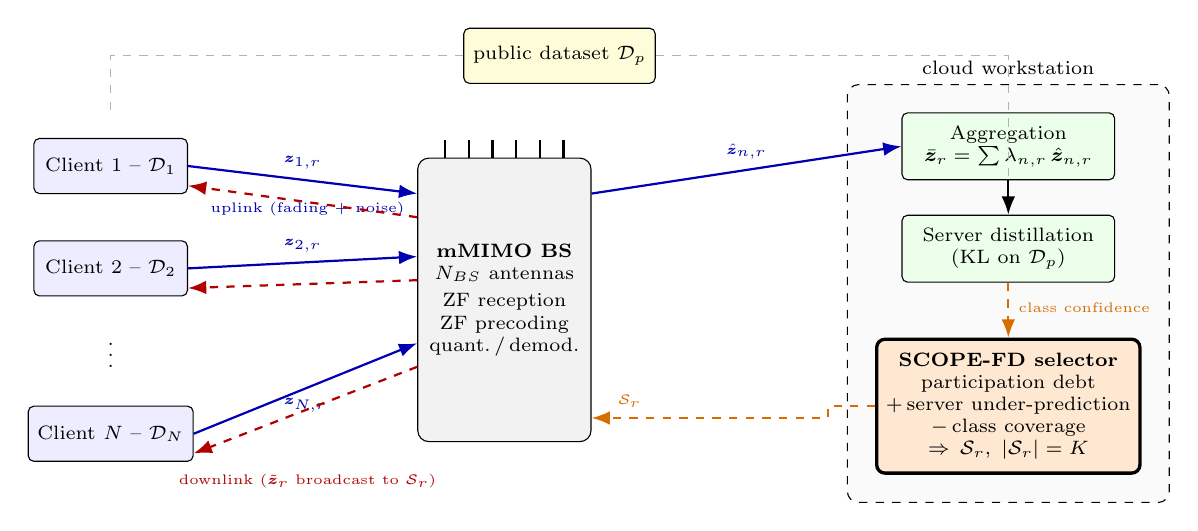
\begin{tikzpicture}[
    font=\footnotesize, >=Latex,
    client/.style  ={draw, rounded corners=2pt, minimum height=0.7cm, minimum width=1.95cm, align=center, fill=blue!7,    font=\scriptsize},
    block/.style   ={draw, rounded corners=2pt, minimum height=0.85cm,minimum width=2.7cm, align=center, fill=green!8,   font=\scriptsize},
    scopebox/.style={draw, rounded corners=3pt, minimum height=1.7cm, minimum width=3.2cm, align=center, fill=orange!18, very thick, font=\scriptsize},
    bs/.style      ={draw, rounded corners=4pt, minimum height=3.6cm, minimum width=2.2cm, align=center, fill=gray!10,   font=\scriptsize},
    pub/.style     ={draw, rounded corners=2pt, minimum height=0.7cm, minimum width=2.3cm, align=center, fill=yellow!15, font=\scriptsize}
]

% --- Clients ---
\node[client] (c1) at (0,  2.6) {Client $1$ -- $\mathcal{D}_1$};
\node[client] (c2) at (0,  1.3) {Client $2$ -- $\mathcal{D}_2$};
\node[font=\scriptsize] at (0, 0.3) {$\vdots$};
\node[client] (cn) at (0, -0.8) {Client $N$ -- $\mathcal{D}_N$};

% --- mMIMO BS ---
\node[bs] (bs) at (5.0, 0.9) {\textbf{mMIMO BS}\\$N_{BS}$ antennas\\[2pt]ZF reception\\ZF precoding\\quant.\,/\,demod.};
\foreach \x in {-0.75,-0.45,-0.15,0.15,0.45,0.75}
  \draw[thick] ($(bs.north)+(\x,0)$) -- ++(0, 0.22);

% --- Public dataset ---
\node[pub] (pub) at (5.7, 4.0) {public dataset $\mathcal{D}_p$};

% --- Cloud workstation contents ---
\node[block] (agg)  at (11.4,  2.85) {Aggregation\\$\bar{\bm{z}}_r=\sum\lambda_{n,r}\,\hat{\bm{z}}_{n,r}$};
\node[block] (dist) at (11.4,  1.55) {Server distillation\\(KL on $\mathcal{D}_p$)};
\node[scopebox] (sel) at (11.4, -0.45) {\textbf{SCOPE-FD selector}\\participation debt\\$+\,$server under-prediction\\$-\,$class coverage\\$\Rightarrow\,\mathcal{S}_r,\;|\mathcal{S}_r|=K$};

% --- Cloud bounding box ---
\begin{scope}[on background layer]
  \node[draw, dashed, rounded corners=4pt, fit=(agg)(dist)(sel), inner sep=10pt, fill=gray!4,
        label={[font=\scriptsize]above:cloud workstation}] (cloud) {};
\end{scope}

% --- UL arrows: clients -> BS (solid blue) ---
\draw[->, thick, blue!70!black] (c1.east) -- node[midway, above, font=\tiny]{$\bm{z}_{1,r}$} ($(bs.west)+(0, 1.35)$);
\draw[->, thick, blue!70!black] (c2.east) -- node[midway, above, font=\tiny]{$\bm{z}_{2,r}$} ($(bs.west)+(0, 0.55)$);
\draw[->, thick, blue!70!black] (cn.east) -- node[midway, below, font=\tiny]{$\bm{z}_{N,r}$} ($(bs.west)+(0,-0.55)$);
\node[font=\tiny, blue!70!black] at (2.5, 2.05) {uplink (fading + noise)};

% --- DL arrows: BS -> clients (dashed red) ---
\draw[->, thick, red!70!black, dashed] ($(bs.west)+(0, 1.05)$) -- ($(c1.east)+(0,-0.25)$);
\draw[->, thick, red!70!black, dashed] ($(bs.west)+(0, 0.25)$) -- ($(c2.east)+(0,-0.25)$);
\draw[->, thick, red!70!black, dashed] ($(bs.west)+(0,-0.85)$) -- ($(cn.east)+(0,-0.25)$);
\node[font=\tiny, red!70!black] at (2.5, -1.4) {downlink ($\tilde{\bm{z}}_r$ broadcast to $\mathcal{S}_r$)};

% --- BS -> Aggregation (recovered logits) ---
\draw[->, thick, blue!70!black] ($(bs.east)+(0, 1.35)$) -- node[midway, above, font=\tiny]{$\hat{\bm{z}}_{n,r}$} (agg.west);

% --- Aggregation -> Distillation ---
\draw[->, thick] (agg.south) -- (dist.north);

% --- Distillation -> SCOPE selector (feedback) ---
\draw[->, thick, orange!85!black, dashed] (dist.south) -- node[right, font=\tiny, pos=0.45]{class confidence} (sel.north);

% --- SCOPE selector -> BS (scheduling decision) ---
\draw[->, thick, orange!85!black, dashed]
   (sel.west) -- ++(-0.6,0) |- ($(bs.east)+(0,-1.5)$)
   node[font=\tiny, pos=0.92, above]{$\mathcal{S}_r$};

% --- Public dataset connections (thin grey, dashed) ---
\draw[dashed, gray!60] (pub.west) -| ($(c1.north)+(0, 0.3)$);
\draw[dashed, gray!60] (pub.east) -| ($(dist.north)+(0, 0.4)$);

\end{tikzpicture}
\caption{Architecture of the proposed SCOPE-FD framework over an mMIMO wireless backbone. $\mathcal{D}_n$ and $\mathcal{D}_p$ are the private and public datasets; $\bm{z}_{n,r}$, $\hat{\bm{z}}_{n,r}$, and $\tilde{\bm{z}}_r$ denote the uplink logits, the ZF-equalized logits at the BS, and the post-distillation logits broadcast over the downlink, respectively. The cloud workstation is the back-end compute node co-located with the BS over a wired (non-communication-budgeted) link, hosting the server-side model, the distillation step, and the SCOPE-FD selector; the only over-the-air segment is the BS-to-client wireless interface. Solid blue arrows denote the uplink streams, dashed red arrows the downlink broadcast, and dashed orange arrows the control path that returns the next-round subset $\mathcal{S}_r$ to the BS.}
\label{fig:system_model}
\end{figure*}

\subsection{Federated Distillation Setup}
\label{ssec:fd-setup}

Consider an FD system where a base station (BS) equipped with $N_{BS}$ antennas serves $N$ single-antenna clients over an mMIMO wireless backbone. The $n^{\text{th}}$ client holds a private local dataset $\mathcal{D}_n = \{(\bm{x}_i, y_i)\}_{i=1}^{|\mathcal{D}_n|}$, where $\bm{x}_i$ is the input sample and $y_i \in \{1, \dots, C\}$ is the corresponding class label. The local datasets are kept private and are not shared with the BS at any stage of training. To capture the data heterogeneity inherent to edge deployments, the per-class proportions on each client are sampled from a Dirichlet distribution $\text{Dir}(\alpha)$ over the label space \cite{hsu2019measuring}, with smaller values of $\alpha$ producing more skewed partitions. A public unlabeled dataset $\mathcal{D}_p = \{\bm{x}_p\}_{p=1}^{|\mathcal{D}_p|}$ is shared by the BS and all clients, and serves as the substrate over which the per-client logits are computed and exchanged \cite{itahara2023distillation}. Since only logits are transmitted, the clients are free to adopt heterogeneous local architectures \cite{chan2021fedhe}.

The local loss at client $n$ is given by
\begin{equation}
L_n(\bm{w}_n) = \frac{1}{|\mathcal{D}_n|} \sum_{(\bm{x}_i, y_i) \in \mathcal{D}_n} \ell(\bm{w}_n; \bm{x}_i, y_i),
\label{eq:local_loss}
\end{equation}
where $\bm{w}_n$ denotes the local model parameters and $\ell(\cdot)$ is the per-sample cross-entropy. The server-side objective is to minimize the data-size-weighted sum of the local losses, namely
\begin{equation}
\min_{\{\bm{w}_n\}} \; F\!\left(\{\bm{w}_n\}\right) = \sum_{n=1}^{N} \frac{|\mathcal{D}_n|}{|\mathcal{D}|} L_n(\bm{w}_n),
\label{eq:global_obj}
\end{equation}
where $|\mathcal{D}| = \sum_{n=1}^{N} |\mathcal{D}_n|$. Following \cite{mu2024fedtskd}, each communication round $r$ consists of three stages, viz., local training, uplink communication and server-side aggregation, and downlink broadcast and local distillation. The overall architecture, including the proposed selector at the cloud workstation, is summarized in Fig.~\ref{fig:system_model}.

In the local training stage, every client $n \in \mathcal{S}_r$ runs $K_r$ steps of stochastic gradient descent (SGD) on its private dataset, where $\mathcal{S}_r$ denotes the set of clients selected in round $r$. The updated local parameters are then used to compute the per-sample logits $\bm{z}_{n,r}$ on the public dataset $\mathcal{D}_p$. After quantization and modulation, the logits are uploaded to the BS through the mMIMO uplink, and the received signal at the BS can be written as
\begin{equation}
\bm{Y}^{(\text{UL})}_{r} = \sum_{n \in \mathcal{S}_r} \bm{H}_{n,r} \bm{Z}_{n,r}^{T} \sqrt{\frac{P_{\text{UL}}}{N_D \sigma_z^2}} + \bm{\Omega}^{(\text{UL})}_{r},
\label{eq:ul_signal}
\end{equation}
where $\bm{Y}^{(\text{UL})}_{r} \in \mathbb{C}^{N_{BS} \times N_D}$ stacks the $N_D$ received symbol periods column-wise, $\bm{H}_{n,r} \in \mathbb{C}^{N_{BS} \times 1}$ is the uplink channel column vector between the single-antenna client $n$ and the $N_{BS}$-antenna BS, $\bm{Z}_{n,r} \in \mathbb{C}^{N_D \times 1}$ is the complex-valued symbol representation of $\bm{z}_{n,r}$ obtained after quantization and modulation, so that $\bm{H}_{n,r}\bm{Z}_{n,r}^{T}$ is the rank-one $N_{BS}\times N_D$ matrix received from client $n$, $P_{\text{UL}}$ is the uplink transmit power in linear scale, $N_D$ is the number of complex data streams per logit vector, $\sigma_z^2$ is the per-symbol average power normalization in linear scale, and $\bm{\Omega}^{(\text{UL})}_{r}$ is the receiver-side complex Gaussian noise. The scaling factor $\sqrt{P_{\text{UL}}/(N_D \sigma_z^2)}$ in (\ref{eq:ul_signal}) splits $P_{\text{UL}}$ uniformly across the $N_D$ data streams and normalizes each entry of $\bm{Z}_{n,r}$ to unit average power, so the per-symbol transmit energy equals $P_{\text{UL}}/N_D$. With zero-forcing (ZF) reception, the per-client logits at the BS can be recovered as
\begin{equation}
\hat{\bm{z}}_{n,r} = \bm{z}_{n,r} + \bm{\omega}^{(\text{UL})}_{n,r},
\label{eq:ul_zf}
\end{equation}
where the variance of the post-equalization noise $\bm{\omega}^{(\text{UL})}_{n,r}$ is suppressed by a factor proportional to $N_{BS}$, owing to the channel hardening property of the mMIMO array \cite{mu2024fedtskd}, \cite{vu2020cell}.

\subsection{FD Aggregation under Partial Participation}
\label{ssec:fd-aggregation}

After dequantization and demodulation at the BS, the round-$r$ aggregated logit is formed by data-size-weighted averaging over the selected clients, that is,
\begin{equation}
\bar{\bm{z}}_r = \sum_{n \in \mathcal{S}_r} \lambda_{n,r} \, \hat{\bm{z}}_{n,r}, \quad \lambda_{n,r} = \frac{|\mathcal{D}_n|}{\sum_{j \in \mathcal{S}_r} |\mathcal{D}_j|}.
\label{eq:agg}
\end{equation}
The server-model parameters are then updated through a distillation step that minimizes the Kullback-Leibler divergence between the server-model output and $\bar{\bm{z}}_r$ on the public dataset \cite{hinton2015distilling}. The post-distillation logits are subsequently quantized, modulated, precoded with a zero-forcing precoder, and broadcast to the selected clients over the mMIMO downlink. Each selected client then performs a local distillation step that updates its local model. As in the uplink, the downlink post-equalization noise variance is suppressed by the channel hardening of the mMIMO array \cite{mu2024fedtskd}.

Once $\mathcal{S}_r$ is fixed, $\bar{\bm{z}}_r$ depends on the per-client logits only through the data-size weights $\lambda_{n,r}$, so the over-round composition of $\mathcal{S}_r$ rather than any within-round client utility drives the progression of the server model. The proposed selector exploits this by directly shaping the over-round composition of $\mathcal{S}_r$.

\subsection{Participation Fairness and Problem Statement}
\label{ssec:problem-statement}

To quantify the per-client participation fairness, the Gini coefficient over the cumulative participation counts is adopted. After $R$ rounds, let $n_i^{(R)}$ denote the total number of rounds in which client $i$ has been selected. The participation Gini coefficient is given by
\begin{equation}
G^{(R)} = \frac{\sum_{i,j} \left|n_i^{(R)} - n_j^{(R)}\right|}{2N \sum_{i=1}^{N} n_i^{(R)}}.
\label{eq:gini}
\end{equation}
A perfectly balanced selection policy yields $G^{(R)} = 0$, whereas uniform random selection yields $G^{(R)} > 0$, with the imbalance growing as the participation ratio $K/N$ shrinks.

The goal of this work is to design a selection policy $\pi$ that returns $\mathcal{S}_r \subset \{1, \dots, N\}$ with $|\mathcal{S}_r| = K$ in each round $r$, so as to minimize the FD convergence error while keeping the participation Gini coefficient small. Letting $\{\bm{w}_n^{(R)}\}$ denote the local model parameters after $R$ rounds under policy $\pi$, the problem can be formulated as
\begin{equation}
\min_{\pi} \; \mathbb{E}\!\left[F\!\left(\{\bm{w}_n^{(R)}\}\right)\right] - F^{*},
\label{eq:problem}
\end{equation}
subject to the following three constraints. First, $|\mathcal{S}_r| = K$ for all $r$, which fixes the per-round communication budget. Second, the selection rule does not require any uplink communication beyond the FedTSKD logit-exchange budget \cite{mu2024fedtskd}; that is, no additional uplink slots are spent on selection-related signalling. Third, the per-round computation at the BS is no greater than $\mathcal{O}(NKC)$ in the number of clients, selection slots, and label classes, so that the selector remains light enough to be executed in every round. Here, $F(\cdot)$ is the global objective defined in (\ref{eq:global_obj}) and $F^{*}$ is its optimal value.

% ============================================================================
% SECTION IV: PROPOSED SCOPE-FD ALGORITHM
% ============================================================================
\section{Proposed SCOPE-FD Algorithm}
\label{sec:scope-alg}

This section presents the proposed SCOPE-FD selector, which combines a participation-debt term, a server under-prediction bonus, and a class-coverage penalty into a single deterministic score, followed by the algorithm summary at the end of the section.

\subsection{Three-Term Selection Score}
\label{ssec:three-term-score}

For each candidate client $i$ at round $r$, the SCOPE-FD score is given by
\begin{equation}
\text{score}_i^{(r,k)} = \tilde{d}_i^{(r)} + \alpha_u\, b_i^{(r)} - \alpha_d\, p_i^{(r,k)},
\label{eq:score}
\end{equation}
where $\tilde{d}_i^{(r)}$ is the participation-debt term, $b_i^{(r)}$ is the server under-prediction bonus, $p_i^{(r,k)}$ is the class-coverage penalty evaluated at the $k$-th greedy slot, and $\alpha_u, \alpha_d \ge 0$ are scalar coefficients that are kept fixed across all configurations. The selector fills the $K$ slots of $\mathcal{S}_r$ greedily, in decreasing order of (\ref{eq:score}); after each pick, the coverage vector that drives $p_i^{(r,k)}$ is updated, while the debt and bonus terms remain fixed within the round. Setting $\alpha_u = \alpha_d = 0$ reduces the selector to deterministic round-robin over the debt rotation; the contribution of this paper is the demonstration that round-robin equipped with two principled tie-breaker terms is sufficient to dominate the random baseline in the FD setting.

\subsection{Participation-Debt Term}
\label{ssec:debt-term}

The participation-debt term is the primary signal of the selector and drives the over-round fairness of SCOPE-FD. Let $n_i^{(r-1)}$ denote the cumulative participation count of client $i$ over the first $r-1$ rounds. The uniform target after $r$ rounds is $r\cdot K/N$, that is, the count each client would have accumulated if every previous selection had been distributed uniformly across the pool. The per-client raw debt is the deviation between this target after round $r$ and the actual count through round $r-1$, namely
\begin{equation}
d_i^{(r)} = r\cdot \frac{K}{N} - n_i^{(r-1)}.
\label{eq:debt}
\end{equation}
A positive value of $d_i^{(r)}$ indicates that client $i$ has been picked less often than the uniform target by the end of round $r-1$ and is therefore a candidate for selection in round $r$, while a negative value indicates over-picking. The raw debt is then mapped to the unit interval through min-max normalization across the candidate pool,
\begin{equation}
\tilde{d}_i^{(r)} = \frac{d_i^{(r)} - \min_j d_j^{(r)}}{\max_j d_j^{(r)} - \min_j d_j^{(r)} + \varepsilon},
\label{eq:debt_norm}
\end{equation}
where $\varepsilon$ is a small positive constant added for numerical stability. Under (\ref{eq:debt_norm}), the most under-picked client of the round always receives $\tilde{d}_i^{(r)} = 1$ and the most over-picked client receives $\tilde{d}_i^{(r)} = 0$, so the debt term spans the full $[0,1]$ range regardless of the magnitude of the raw debt. The participation history needed to evaluate (\ref{eq:debt}) is already maintained at the BS as a by-product of scheduling and does not require any additional client-side signalling.

\subsection{Server Under-Prediction Bonus}
\label{ssec:bonus-term}

\revIVE{The server under-prediction bonus is a secondary signal that tilts the selection towards clients whose local data covers classes the server model currently under-predicts on the public dataset.} Let $\bm{u}^{(r)} \in \mathbb{R}^{C}$ denote the per-class under-prediction vector at round $r$, whose $c$-th entry is one minus the average softmax mass the server places on class $c$ across $\mathcal{D}_p$, namely
\begin{equation}
u_c^{(r)} = 1 - \frac{1}{|\mathcal{D}_p|}\sum_{p=1}^{|\mathcal{D}_p|} \mathrm{softmax}_c\!\left(g(\bm{x}_p; \bm{\theta}_r)\right),
\label{eq:uncert}
\end{equation}
where $\bm{\theta}_r$ denotes the server-model parameters at the start of round $r$ (i.e., after the round-$(r{-}1)$ distillation step in \cite[Algorithm~1]{mu2024fedtskd}) and $g(\bm{x}_p; \bm{\theta}_r) \in \mathbb{R}^{C}$ is the corresponding server-model logit on the public sample $\bm{x}_p$. \revIVE{A high value of $u_c^{(r)}$ indicates that class $c$ is rarely predicted by the server on $\mathcal{D}_p$, whether due to genuine uncertainty, class bias, or a skewed public-data prior; the bonus does not distinguish between these causes.} Letting $\bm{h}_i \in \mathbb{R}^{C}$ denote the L1-normalized label histogram of client $i$, the bonus is given by
\begin{equation}
b_i^{(r)} = \langle \bm{h}_i, \bm{u}^{(r)} \rangle = \sum_{c=1}^{C} h_{i,c}\, u_c^{(r)}.
\label{eq:bonus}
\end{equation}
\revIVE{The score is therefore biased towards clients whose histograms overlap with the under-predicted classes, targeting regions of the label space the server has not yet learnt to recover. The vector $\bm{u}^{(r)}$ is computed at the cloud workstation from softmax outputs already produced during the distillation step, so no extra uplink communication is incurred. Each $\bm{h}_i$ is uploaded once at session initialization; the resulting $\mathcal{O}(C)$ per-client overhead is dominated by a single round of logit exchange.}

\subsection{Class-Coverage Penalty}
\label{ssec:penalty-term}

The class-coverage penalty discourages picking a client whose label distribution overlaps heavily with the classes already covered by the partial selection $\mathcal{S}_r^{(<k)}$ at the $k$-th greedy slot. Let $\bm{c}^{(r,k)} \in [0,1]^{C}$ denote the per-class coverage vector at the start of slot $k$, defined as
\begin{equation}
c_{j}^{(r,k)} = \min\!\left(1,\, \sum_{n \in \mathcal{S}_r^{(<k)}} h_{n,j}\right),
\label{eq:cov}
\end{equation}
which saturates at unity once class $j$ has been fully covered by the partial selection. The saturation in (\ref{eq:cov}) prevents the penalty from over-counting classes that are already represented and keeps each entry of $\bm{c}^{(r,k)}$ in $[0,1]$. The coverage penalty for candidate $i$ at slot $k$ is the inner product
\begin{equation}
p_i^{(r,k)} = \langle \bm{h}_i, \bm{c}^{(r,k)} \rangle.
\label{eq:penalty}
\end{equation}
At the first slot of each round, $\bm{c}^{(r,1)} = \bm{0}$ and the penalty is uniformly zero. At subsequent slots, the penalty grows for clients whose histograms overlap with the already-selected classes, so the within-round selection naturally diversifies across the label space.

\new{\textit{Privacy consideration:} Both (\ref{eq:bonus}) and (\ref{eq:penalty}) represent the per-client label histogram $\bm{h}_i$, which discloses the per-class distribution of the local dataset to the server. Towards that, two complementary remedies are compatible with the proposed selector, namely a calibrated Laplace mechanism on the histogram upload, and a server-side softmax-averaged surrogate computed from the per-client public-dataset logits already observed in (\ref{eq:agg}) once each client has been selected at least once. A quantitative characterisation of either remedy on the FD pipeline is left to future investigation.}

\rev{\textit{Choice of the coefficients.} The non-negative coefficients $\alpha_u, \alpha_d \ge 0$ in (\ref{eq:score}) are kept fixed across all configurations, with $(\alpha_u, \alpha_d) = (0.3, 0.1)$ used throughout Section~\ref{sec:experiments}. The values are not tuned for accuracy. They are chosen so that the participation-debt term remains the dominant signal, which is the condition under which Proposition~1 holds. The normalized debt in (\ref{eq:debt_norm}) lies in $[0,1]$ and changes by one full unit between a client that is one round behind and a client that is level. The bonus in (\ref{eq:bonus}) and the penalty in (\ref{eq:penalty}) are also bounded in $[0,1]$ by construction. Their combined influence is therefore at most $\alpha_u + \alpha_d$, and any setting with $\alpha_u + \alpha_d < 1$ leaves the debt ordering intact while allowing the two information terms to break ties inside a debt-equal cohort. The setting $(0.3, 0.1)$ sits comfortably inside this region.

This reasoning is verified empirically in Section~\ref{ssec:exp-coefgrid}, where a grid over $\alpha_u$ and $\alpha_d$ shows that the participation Gini coefficient is unchanged across every admissible setting and that the final accuracy varies by little more than one percentage point over the whole grid.}

\subsection{Algorithm Summary and Complexity}
\label{ssec:algorithm-summary}

Algorithm~\ref{alg:scopefd} summarizes the proposed SCOPE-FD selector at the BS. In the first round, all participation counts are zero and the debt is uniform; the selection therefore reduces to picking $K$ clients by the bonus minus the penalty alone. From the second round onward, the debt term dominates the score and drives the over-round rotation, with the bonus and penalty acting as tie-breakers within debt-equal cohorts.

\begin{algorithm}[t]
\caption{\small SCOPE-FD Selector at Round $r$}
\label{alg:scopefd}
\begin{algorithmic}[1]
\small
\REQUIRE Round index $r$, slot count $K$, label histograms $\{\bm{h}_i\}$, participation counts $\{n_i^{(r-1)}\}$;
\REQUIRE Under-prediction vector $\bm{u}^{(r)}$, coefficients $\alpha_u, \alpha_d$
\ENSURE Selected subset $\mathcal{S}_r$ with $|\mathcal{S}_r|=K$
\STATE Compute $\tilde{d}_i^{(r)}$ for all $i$ via (\ref{eq:debt})--(\ref{eq:debt_norm})
\STATE Compute $b_i^{(r)}$ for all $i$ via (\ref{eq:bonus})
\STATE Initialize $\mathcal{S}_r \leftarrow \emptyset$ and $\bm{c}^{(r,1)} \leftarrow \bm{0}$
\FOR{$k = 1$ to $K$}
    \STATE Compute $p_i^{(r,k)}$ for all $i \notin \mathcal{S}_r$ via (\ref{eq:penalty})
    \STATE $i^{*} \leftarrow \arg\max\limits_{i \notin \mathcal{S}_r}\;\tilde{d}_i^{(r)} + \alpha_u b_i^{(r)} - \alpha_d p_i^{(r,k)}$ (ties broken by smallest client index)
    \STATE $\mathcal{S}_r \leftarrow \mathcal{S}_r \cup \{i^{*}\}$
    \STATE Update $\bm{c}^{(r,k+1)}$ via (\ref{eq:cov})
\ENDFOR
\RETURN $\mathcal{S}_r$
\end{algorithmic}
\end{algorithm}

The per-round computational cost at the BS is $\mathcal{O}(NKC)$: the debt and bonus terms cost $\mathcal{O}(NC)$, and the greedy outer loop runs $K$ iterations with $\mathcal{O}(NC)$ per iteration for the coverage penalty. The memory footprint is $\mathcal{O}(NC)$, dominated by the per-client label histograms. Both complexities are linear in $N$ for fixed $K$ and $C$, satisfying the third constraint in Section~\ref{ssec:problem-statement}.

% ============================================================================
% SECTION V: THEORETICAL ANALYSIS
% ============================================================================
\section{Theoretical Analysis}
\label{sec:theory}

This section presents the theoretical analysis of SCOPE-FD. The window-wise participation-balance guarantee is established first, followed by the compatibility with the convergence bound of FedTSKD \cite{mu2024fedtskd}.

\subsection{Participation-Balance Guarantee}
\label{ssec:participation-balance}

\textit{Proposition 1 (Bounded Participation Spread):} Under the SCOPE-FD selector with non-negative coefficients $\alpha_u, \alpha_d$ such that $\alpha_u + \alpha_d < 1$, which is satisfied by the calibration $(0.3, 0.1)$ used in this paper, the per-client cumulative participation counts after any $R$ rounds satisfy
\begin{equation}
\left| n_i^{(R)} - n_j^{(R)} \right| \le 1, \qquad \forall\, i,j \in \{1,\dots,N\},
\label{eq:spread}
\end{equation}
that is, no two clients differ by more than one in their cumulative participation. The participation Gini coefficient is consequently bounded by
\begin{equation}
G^{(R)} \le \frac{N}{4KR},
\label{eq:gini_bound}
\end{equation}
which decays as $\mathcal{O}(1/R)$ for fixed $N$ and $K$.

\textit{Proof sketch:} The argument proceeds by induction on the round index $r$. The base case $r = 1$ is trivial since all participation counts are zero. For the inductive step, assume $|n_i^{(r-1)} - n_j^{(r-1)}| \le 1$ at the start of round $r$, and let $L = \min_i n_i^{(r-1)}$, so the round-start counts lie in $\{L, L+1\}$; call the cohorts with these two counts \emph{under-picked} and \emph{over-picked}, respectively. The raw debts (\ref{eq:debt}) take exactly two values that differ by one, and the min-max normalization (\ref{eq:debt_norm}) sends the under-picked cohort to $\tilde{d}_i^{(r)} = 1/(1+\varepsilon)$ and the over-picked cohort to $\tilde{d}_i^{(r)} = 0$, \revIVE{where $\varepsilon$ is taken small enough that $1/(1+\varepsilon) > \alpha_u + \alpha_d$, a condition met by orders of magnitude at the calibration $(0.3, 0.1)$ for any standard numerical floor.} Since $b_i^{(r)}, p_i^{(r,k)} \in [0,1]$, the score gap between any under-picked and any over-picked client is therefore at least $1/(1+\varepsilon) - (\alpha_u + \alpha_d) > 0$. \revIVE{Because $\tilde{d}_i^{(r)}$ is held fixed within the round and the bound on $p_i^{(r,k)}$ is slot-independent, the gap holds uniformly across all $K$ greedy slots,} so the greedy filling picks all under-picked clients before any over-picked one. If the under-picked cohort has size $\ge K$, all $K$ picks are drawn from it and the round-end counts again lie in $\{L, L+1\}$. Otherwise all under-picked clients are picked together with a subset of the over-picked cohort, after which the originally under-picked clients are at $L+1$, the picked over-picked clients at $L+2$, and the unpicked over-picked clients at $L+1$; the round-end counts therefore lie in $\{L+1, L+2\}$. Either way the spread is one and (\ref{eq:spread}) holds, completing the induction. For the Gini bound, if $a$ clients end at $L$ and $N-a$ at $L+1$, the numerator of (\ref{eq:gini}) equals $2a(N-a) \le N^2/2$ and the denominator equals $2NKR$, which yields (\ref{eq:gini_bound}). \hfill$\blacksquare$

When $N$ is an integer multiple of $K$, the cycle length $\lceil N/K \rceil = N/K$ corresponds to exactly $N$ selection slots, and (\ref{eq:spread}) sharpens to equality of all participation counts at the end of each cycle. The participation Gini coefficient is then identically zero over every $N/K$-round window, irrespective of the channel state and the Dirichlet heterogeneity level $\alpha$, starting from the standard zero-initialised participation counts.

\rev{The divisibility condition $K \mid N$ is required only for the sharpened statement. The bound (\ref{eq:spread}) itself is proved without it, so the guarantee does not break when $K \nmid N$. What changes is that the total number of selection slots after $R$ rounds, namely $KR$, need not be an integer multiple of $N$. The counts then settle on two adjacent integers rather than one, and the residual Gini coefficient is governed by (\ref{eq:gini_bound}), which continues to decay as $\mathcal{O}(1/R)$. The same reasoning applies to an evaluation window that does not begin and end on a cycle boundary, since the spread bound holds at every round and not only at cycle ends. Both cases are examined empirically in Section~\ref{ssec:exp-scale}.}

Proposition~1 governs participation balance only. The bonus and penalty terms enter the score strictly within the debt-equal cohort and therefore do not affect the spread bound (\ref{eq:spread}); their role in the FD pipeline is to refine the within-round composition of $\mathcal{S}_r$ rather than to alter its over-round count distribution. %Any utility-axis comparison against utility-driven selectors operating outside the FD aggregation rule is left to future work.

\subsection{Compatibility with the FedTSKD Convergence Bound}
\label{ssec:convergence-compat}

The proposed selector modifies only the composition of $\mathcal{S}_r$ at each round, while the local training, server-side aggregation, and distillation steps of FedTSKD \cite{mu2024fedtskd} remain unchanged. The convergence guarantee of FedTSKD therefore continues to hold under SCOPE-FD selection without modification, as captured by the following remark.

\textit{Remark (Convergence-Bound Compatibility):} Let Assumptions 1--4 of \cite{mu2024fedtskd} hold for the local and global loss functions. Under SCOPE-FD selection, the per-client convergence bound of \cite[Theorem~1]{mu2024fedtskd},
\begin{equation}
\mathbb{E}\!\left[L_n\!\left(\bm{w}_{n,t+1}\right)\right] - L_n^{*} \le \frac{\psi}{2}\cdot\frac{\nu_n}{t+1+\beta_1},
\label{eq:conv_bound}
\end{equation}
continues to hold, where $\psi$ is the smoothness constant of the global objective, $\nu_n$ captures the per-client local-gradient variance, and $\beta_1$ is the regularization offset, both as defined in \cite[Theorem~1]{mu2024fedtskd}. The argument is direct: the proof of that theorem invokes the per-round client subset $\mathcal{S}_r$ only through the data-size-weighted aggregation $\bar{\bm{z}}_r$ in (\ref{eq:agg}) and the bounded-variance assumption on the local gradients. SCOPE-FD changes only which subset $\mathcal{S}_r$ enters this aggregation; the local-training process at each client, and hence each client's per-client variance budget $\nu_n$, is unchanged. The aggregator-level argument of \cite{mu2024fedtskd} therefore goes through without modification, with constants depending on the selected cohort size $K$ in place of the full population $N$.

%A tighter analysis that exploits the deterministic nature of the SCOPE-FD selector to refine the constants $\nu_n$ and $\beta_1$ is left to future investigation.

% ============================================================================
% SECTION VI: EXPERIMENTAL RESULTS
% ============================================================================
\section{Experimental Results}
\label{sec:experiments}

The experimental study below evaluates SCOPE-FD as a fairness-first selector and provides a Pareto improvement on the (final accuracy, participation Gini) pair, rather than a uniform accuracy gain.

\subsection{Experimental Setup}
\label{ssec:exp-setup}

The proposed SCOPE-FD selector is integrated into the FedTSKD framework \cite{mu2024fedtskd} and benchmarked against uniform random selection and four ported selectors on Fashion-MNIST (FMNIST). The common simulation parameters are listed in Table~\ref{tab:setup} and mirror those of \cite{mu2024fedtskd} where applicable, with the partial-participation $K$ and the selection-side coefficients $\alpha_u, \alpha_d$ introduced by the present work.

\rev{\textit{Reporting protocol.} Every configuration is repeated over independent seeds and every reported quantity is a mean with a standard deviation over those repetitions. The headline configuration and the selector comparison use five seeds. The parameter sweeps use three seeds. The number of repetitions is stated in each table. Accuracy comparisons between two selectors are supported by a paired Wilcoxon signed-rank test computed over matched seeds, so that the data partition and the channel realization are held fixed within each pair. Convergence speed is reported as the number of rounds required to reach a fixed absolute accuracy threshold, in place of a threshold defined relative to each method's own final accuracy, since the latter is not comparable across methods that converge to different ceilings.} Each client holds a private partition with Dirichlet concentration $\alpha = 0.5$, MNIST is used as the public dataset for logit exchange \cite{itahara2023distillation}, and clients adopt heterogeneous local architectures from the FD-CNN1/2/3 pool \cite{chan2021fedhe}. The mMIMO BS is equipped with $N_{BS} = 64$ antennas, the uplink SNR is fixed at $-8$~dB, and the downlink SNR is varied over $\{\text{error-free}, 0, -10, -20, -30\}$~dB. The distillation temperature is fixed at $T = 1.0$ to match the configuration of the underlying FedTSKD framework \cite{mu2024fedtskd}.%, where the channel-aware aggregation already provides the smoothing that a higher temperature would otherwise contribute; a temperature sweep is left to future investigation. 
FMNIST is the primary benchmark because it offers FD-signal headroom for the selection rule to be observable across both sweeps.%; an extension to CIFAR-10, where the FD accuracy floor under small heterogeneous architectures compresses the selection-axis signal-to-noise, is left to future work. 
In every configuration, SCOPE-FD is paired against uniform random on the same data partition, channel realization, and random seed, so any difference is attributable to the selection rule alone. %The simulation code is planned to be released publicly upon acceptance to support reproducibility.

\begin{table}[t]
\centering
\caption{Common simulation setup, mirroring \cite{mu2024fedtskd}.}
\label{tab:setup}
\renewcommand{\arraystretch}{1.25}
\footnotesize
\setlength{\tabcolsep}{4pt}
\begin{tabular}{@{}>{\raggedright\arraybackslash}m{0.40\columnwidth}>{\raggedright\arraybackslash}m{0.53\columnwidth}@{}}
\toprule
\textbf{Parameter} & \textbf{Value} \\
\midrule
BS antennas $N_{BS}$ & $64$ \\
UL SNR & $-8$ dB \\
DL SNR & $-20$ dB default; swept $\{\text{err-free}, 0, -10, -20, -30\}$ dB \\
Communication rounds $R$ & $100$ \\
Private datasets & FMNIST (primary), MNIST \\
Public dataset & cross-pair (MNIST when FMNIST is private) \\
\rev{Public-set size} & \rev{$2000$ samples} \\
\rev{Client pool $N$} & \rev{$30$ default, swept over $\{47,50,53,100,200\}$} \\
\rev{Cohort size $K$} & \rev{$5$ default, swept over $\{1,3,5,10\}$} \\
Dirichlet $\alpha$ & \rev{$0.5$ default, swept over $\{0.05,0.1,0.3,0.5,1.0,5.0\}$} \\
Client architectures & FD-CNN1 / FD-CNN2 / FD-CNN3 \\
Optimizer & SGD (local), Adam (server distillation) \\
Learning rate & $10^{-2}$ (local), $10^{-3}$ (distillation) \\
Distillation temperature & $1.0$ \\
Logit quantization & $8$-bit \\
SCOPE-FD coefficients & $\alpha_u = 0.3,\ \alpha_d = 0.1$ \\
\rev{Seeds} & \rev{$5$ seeds headline, $3$ seeds sweeps} \\
\bottomrule
\end{tabular}
\end{table}

\rev{\subsection{Ablation of the Score Terms}
\label{ssec:exp-ablation}

The score (\ref{eq:score}) combines three terms, so the first question is how much each one contributes. Four variants are compared at the headline configuration $N=30$, $K=5$, $\alpha=0.5$ over five seeds. The variants are the participation debt alone, the debt with the under-prediction bonus, the debt with the class-coverage penalty, and the complete score. The results are shown in Fig.~\ref{fig:ablation4} and listed in Table~\ref{tab:ablation4}.

\begin{figure}[!t]
\centering
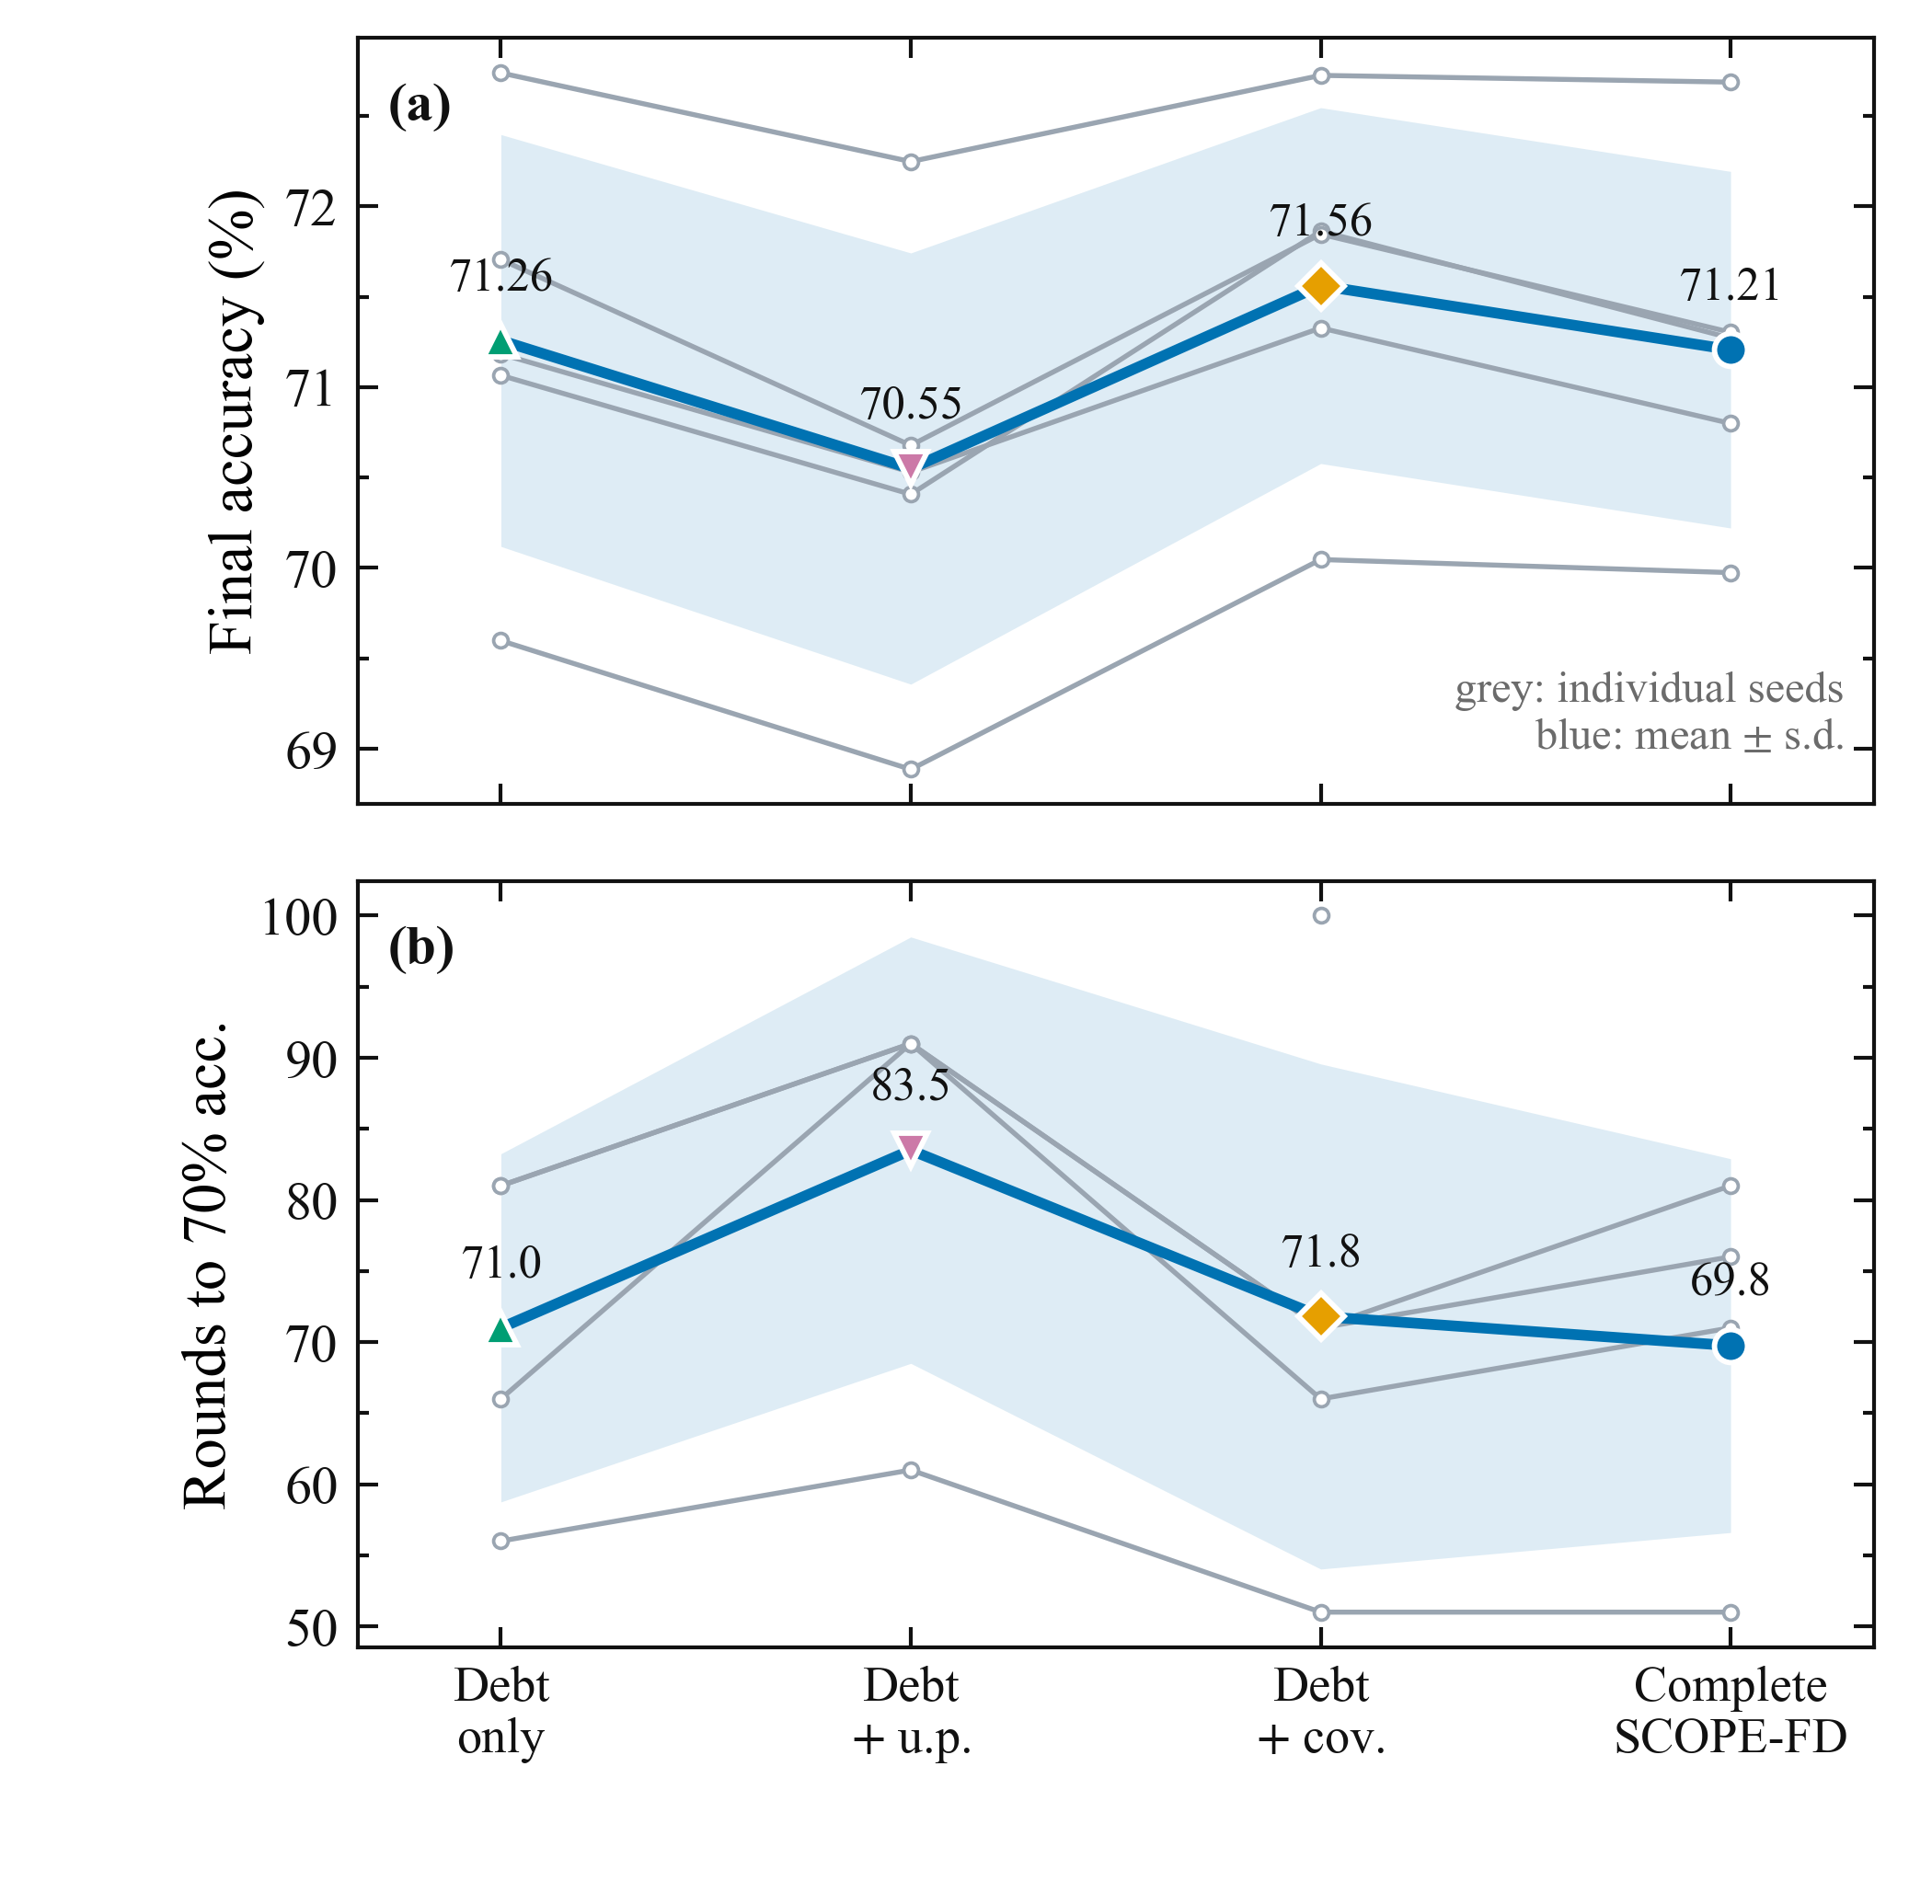
\includegraphics[width=\columnwidth]{figures_revised/fig_r1_ablation_fourway}
\caption{Ablation of the three score terms on FMNIST at $N=30$, $K=5$, $\alpha=0.5$. Each grey trace follows one of the five seeds across the four variants and the blue trace is the mean with one standard deviation. The vertical spread between seeds exceeds the spread between variants, and the seed traces do not reorder consistently, so the four variants cannot be separated on either metric. The participation Gini coefficient is $1.33\%$ for all four.}
\label{fig:ablation4}
\end{figure}

\begin{table}[t]
\centering
\caption{Ablation of the score terms. FMNIST, $N=30$, $K=5$, $\alpha=0.5$, five seeds, mean $\pm$ standard deviation.}
\label{tab:ablation4}
\renewcommand{\arraystretch}{1.15}
\footnotesize
\setlength{\tabcolsep}{4pt}
\begin{tabular}{@{}lccc@{}}
\toprule
\textbf{Variant} & \textbf{Accuracy (\%)} & \textbf{Gini (\%)} & \textbf{Rounds to $70\%$} \\
\midrule
Debt only              & $71.26 \pm 1.14$ & $1.33$ & $71.0$ \\
Debt $+$ under-pred.   & $70.55 \pm 1.19$ & $1.33$ & $83.5$ \\
Debt $+$ coverage      & $71.56 \pm 0.98$ & $1.33$ & $71.8$ \\
Complete SCOPE-FD      & $71.21 \pm 0.99$ & $1.33$ & $69.8$ \\
\bottomrule
\end{tabular}
\end{table}

Two observations follow. First, the participation-debt term supplies the entire fairness result. All four variants reach a Gini coefficient of $1.33\%$, which is the residual predicted by (\ref{eq:gini_bound}) when the number of selection slots is not an exact multiple of $N$. Removing either information term leaves this value unchanged, which is the behaviour Proposition~1 predicts, since those terms act only inside a debt-equal cohort. Second, the four variants are statistically indistinguishable in final accuracy, as the standard deviations in Table~\ref{tab:ablation4} overlap in every pair. The measurable effect of the two information terms is on convergence speed, where the complete score reaches $70\%$ absolute accuracy in $69.8$ rounds against $71.0$ rounds for the debt term alone. This margin is small relative to its spread across seeds. The fairness guarantee is therefore the primary result of the selector, and the two information terms provide a modest refinement of the convergence path rather than an accuracy improvement. The same four-way comparison was repeated across the participation sweep $K \in \{1, 3, 5, 10\}$. The spread between the four variants stays between $0.46$ and $1.58$ percentage points at every $K$, and no variant leads consistently, so the conclusion drawn at the headline configuration is not specific to it.

\subsection{Comparison with Ported Selectors}
\label{ssec:exp-baselines}

The selector is next compared against four published methods ported into the FD pipeline as described in Section~\ref{ssec:rw-fl-selection}, together with uniform random selection and the debt-only variant. Fig.~\ref{fig:baselines} and Table~\ref{tab:baselines} report the results at the headline configuration over five seeds.

\begin{figure}[!t]
\centering
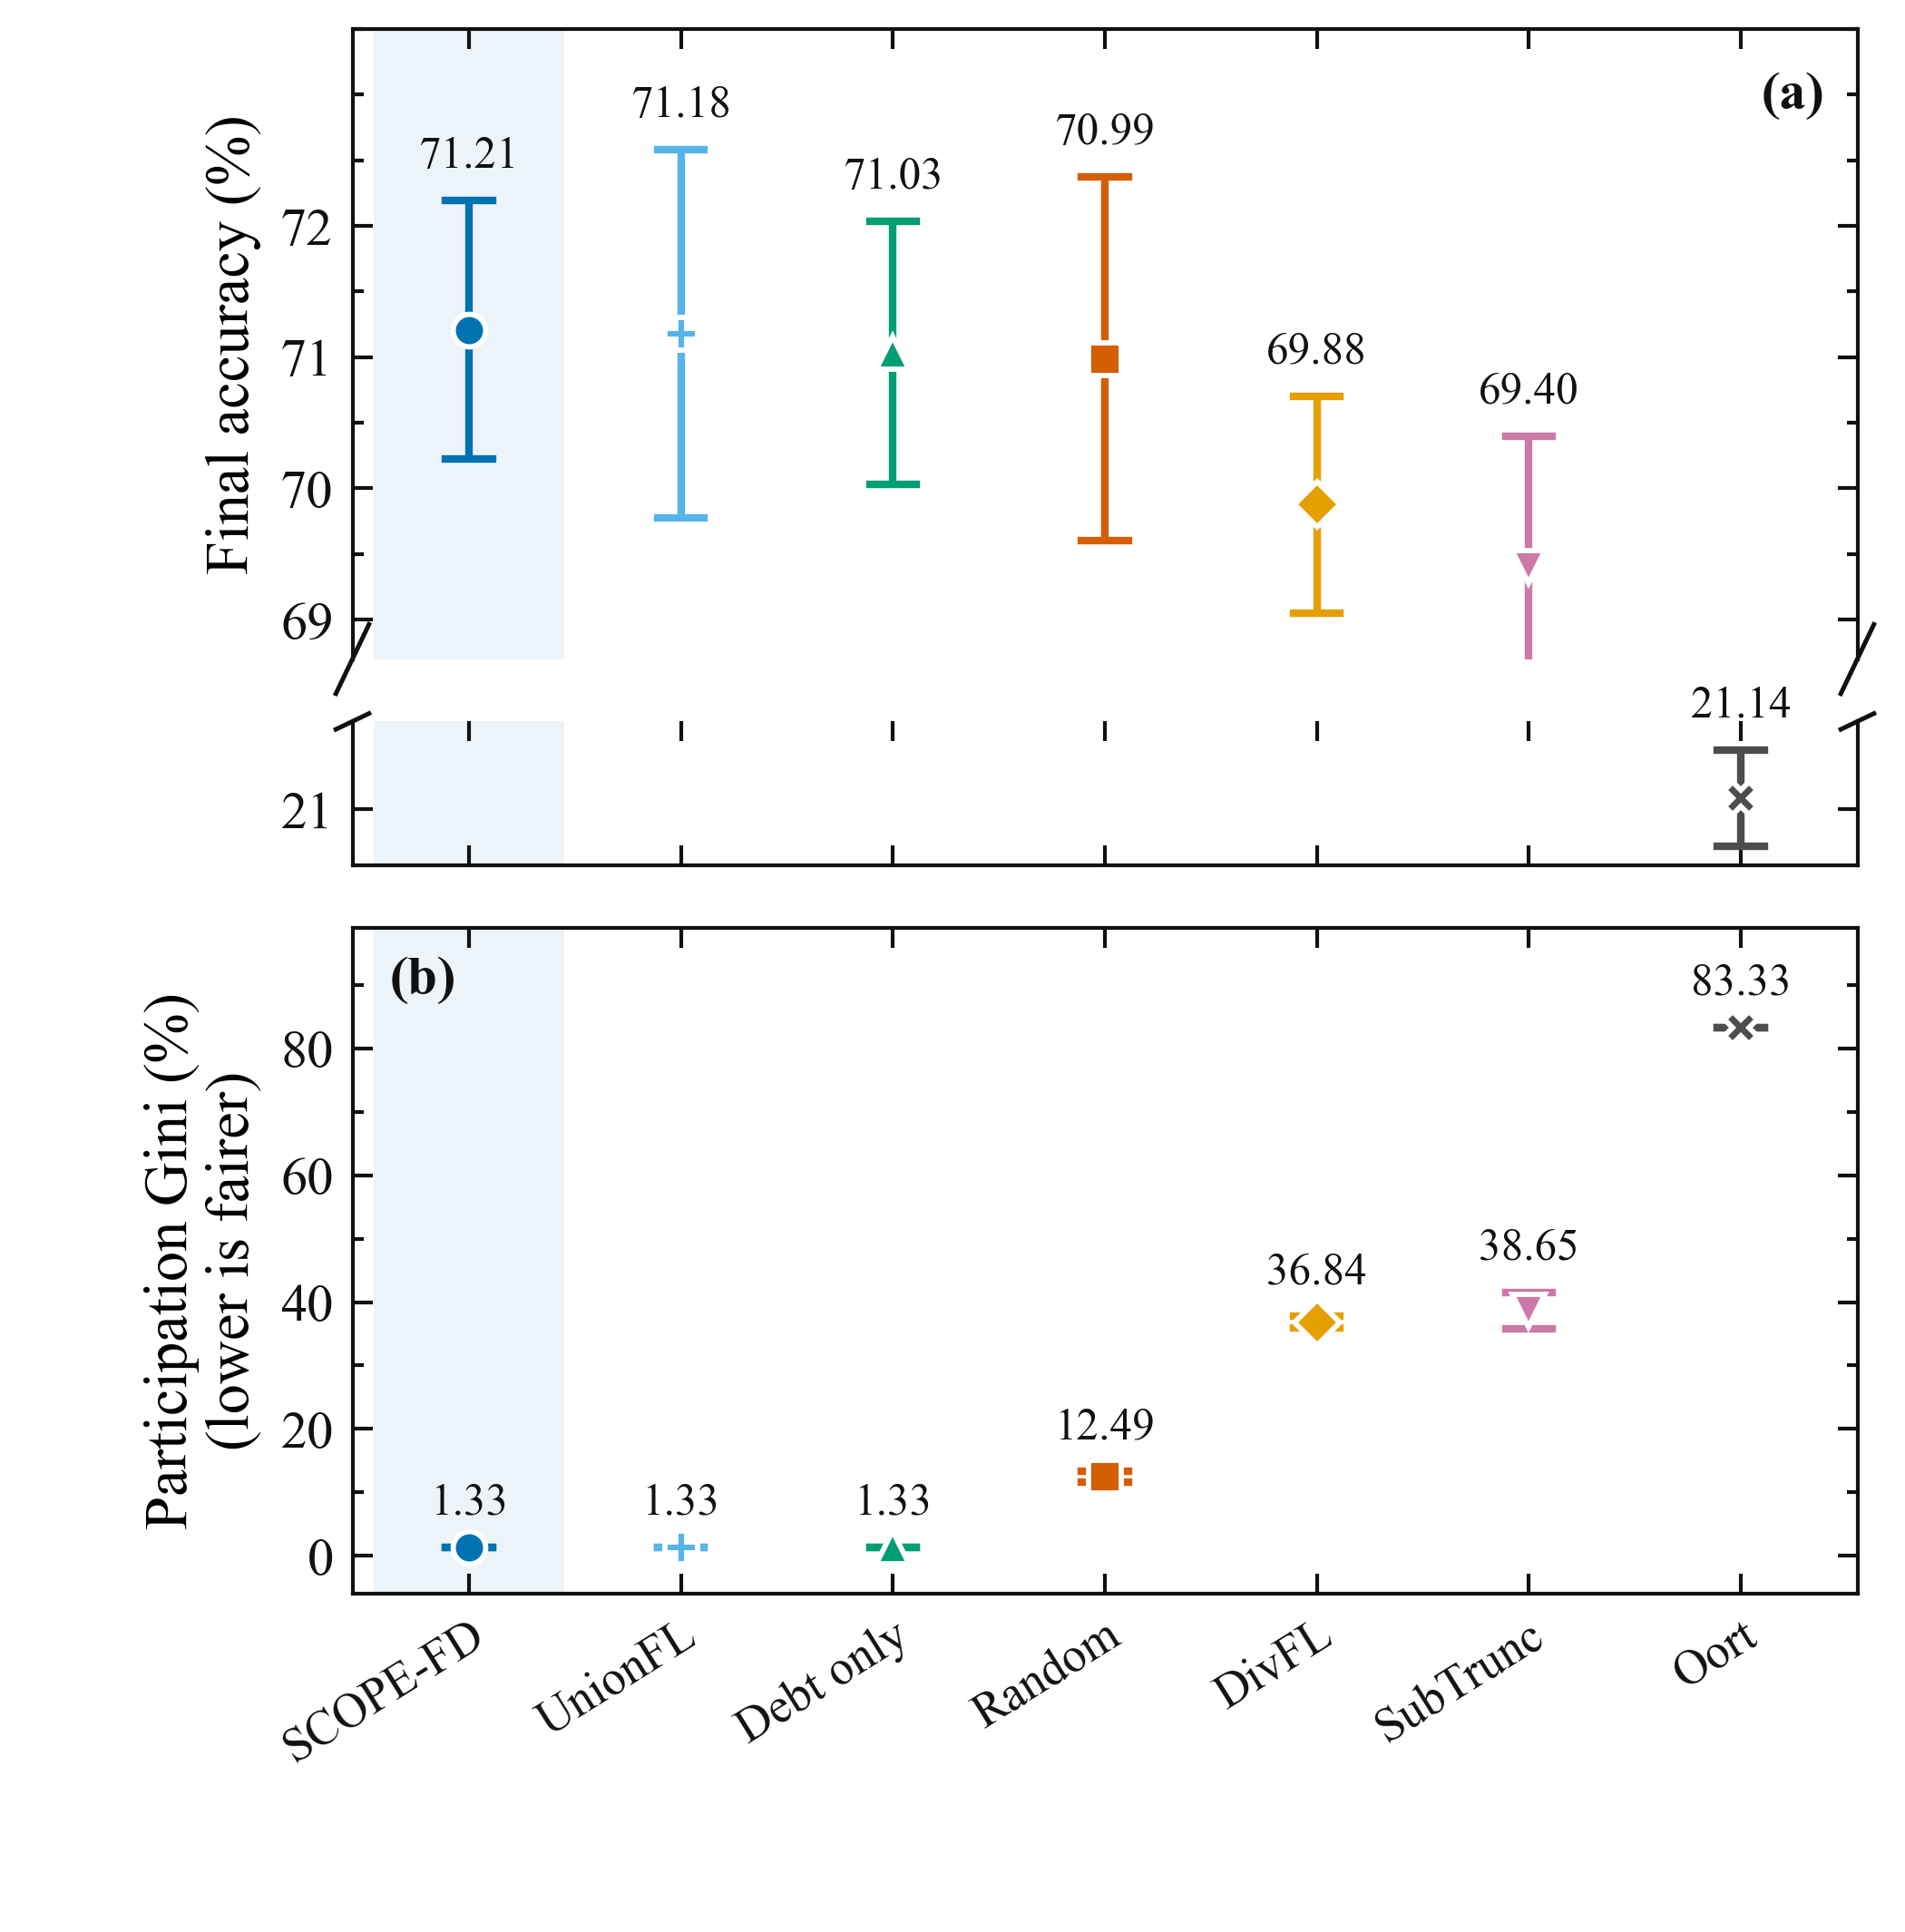
\includegraphics[width=\columnwidth]{figures_revised/fig_r2_baselines}
\caption{Selector comparison on FMNIST at $N=30$, $K=5$, $\alpha=0.5$ over five seeds, ordered by final accuracy with the proposed selector's column shaded. Whiskers are one standard deviation. The accuracy axis in (a) is broken because Oort falls roughly fifty percentage points below every other selector, which would otherwise compress the competitive field into a single line.}
\label{fig:baselines}
\end{figure}

\begin{table}[t]
\centering
\caption{Selector comparison. FMNIST, $N=30$, $K=5$, $\alpha=0.5$, five seeds, mean $\pm$ standard deviation.}
\label{tab:baselines}
\renewcommand{\arraystretch}{1.15}
\footnotesize
\setlength{\tabcolsep}{4pt}
\begin{tabular}{@{}lcc@{}}
\toprule
\textbf{Selector} & \textbf{Accuracy (\%)} & \textbf{Gini (\%)} \\
\midrule
SCOPE-FD (proposed) & $71.21 \pm 0.99$ & $1.33$ \\
Debt only           & $71.03 \pm 1.00$ & $1.33$ \\
UnionFL \cite{castillo2025subtrunc}  & $71.18 \pm 1.40$ & $1.33$ \\
Uniform random      & $70.99 \pm 1.38$ & $12.49$ \\
DivFL \cite{balakrishnan2022divfl}   & $69.88 \pm 0.83$ & $36.84$ \\
SubTrunc \cite{castillo2025subtrunc} & $69.40 \pm 1.00$ & $38.65$ \\
Oort \cite{lai2021oort}              & $21.14 \pm 0.60$ & $83.33$ \\
\bottomrule
\end{tabular}
\end{table}

The proposed selector improves on DivFL by $1.33$ and on SubTrunc by $1.81$ percentage points in final accuracy, and it lowers their participation Gini coefficient by more than an order of magnitude. Against uniform random selection and against UnionFL the accuracy difference lies inside one standard deviation, so the three are treated as tied on that axis, and the separation is in participation fairness alone. The two submodular methods concentrate participation heavily, reaching Gini coefficients above $36\%$, because their diversity objective is evaluated per round and carries no memory of which clients have already been served.

The Oort result is the most informative entry in the table and quantifies the argument of Section~\ref{ssec:rw-fd}. Transferring a utility-based FL selector into FD without modification lowers final accuracy to $21.14 \pm 0.60$, a gap of over fifty percentage points, and raises the Gini coefficient to $83.33\%$. The mechanism is the aggregation rule in (\ref{eq:agg}). A utility-driven rule repeatedly returns to the same high-loss clients, and in FD this narrows the set of clients contributing to the averaged logits, so the distillation target itself becomes biased toward a small subset. In FL the same rule is productive because each selected update enters the parameter average directly. This measurement therefore supports, rather than merely asserts, the claim that FL selection rules do not transfer to FD.

\subsection{Sensitivity to the Selector Coefficients}
\label{ssec:exp-coefgrid}

The magnitude argument of Section~\ref{ssec:three-term-score} predicts that any setting with $\alpha_u + \alpha_d < 1$ preserves the debt ordering. This is tested directly on a grid of $\alpha_u \in \{0, 0.1, 0.2, 0.3, 0.5, 0.8\}$ against $\alpha_d \in \{0, 0.05, 0.1, 0.2, 0.4\}$, giving thirty settings, each repeated over three seeds. The outcome is shown in Fig.~\ref{fig:coefgrid}.

\begin{figure}[!t]
\centering

\includegraphics[width=\columnwidth]{figures_revised/fig_r5_coefficient_grid}
\caption{Sensitivity to the two selector coefficients on FMNIST at $N=30$, $K=5$, three seeds per cell. Final accuracy varies by $1.33$ percentage points across the whole grid and the participation Gini coefficient is $1.33\%$ in every cell.}
\label{fig:coefgrid}
\end{figure}

The participation Gini coefficient is $1.33\%$ in every cell of the grid without exception, which confirms the prediction that the fairness guarantee is independent of the particular admissible values chosen. Final accuracy ranges from $70.94\%$ to $72.27\%$, so the entire grid spans $1.33$ percentage points, which is comparable to the seed-to-seed spread at a single setting. The configuration used throughout this paper, $(\alpha_u, \alpha_d) = (0.3, 0.1)$, reaches $71.99\%$ and sits within half a percentage point of the best cell. The selector therefore does not require the two coefficients to be tuned per configuration.

\subsection{Data Heterogeneity}
\label{ssec:exp-heterogeneity}

The effect of the partition severity is examined by sweeping the Dirichlet concentration over $\alpha \in \{0.05, 0.1, 0.3, 0.5, 1.0, 5.0\}$ at $N=30$, $K=5$. Fig.~\ref{fig:dirichlet} shows the outcome.

\begin{figure*}[!t]
\centering

\includegraphics[width=\textwidth]{figures_revised/fig_r4_dirichlet_severity}
\caption{Effect of the Dirichlet concentration on FMNIST at $N=30$, $K=5$. Shaded bands are one standard deviation over seeds.}
\label{fig:dirichlet}
\end{figure*}

Severe heterogeneity lowers accuracy for every selector alike. At $\alpha = 0.05$ the proposed selector reaches $26.74 \pm 4.19$ and uniform random reaches $27.07 \pm 4.24$, while at $\alpha = 5.0$ the two reach $84.67 \pm 0.11$ and $84.60 \pm 0.18$ respectively. Across the whole range the accuracy difference between the two remains inside one standard deviation. The participation Gini coefficient, in contrast, is $1.33\%$ for the proposed selector and $12.49\%$ for uniform random at every value of $\alpha$ tested. The fairness guarantee is therefore invariant to the degree of data heterogeneity, which is the expected consequence of Proposition~1, since the debt term depends only on participation counts and not on the data distribution. The two submodular baselines degrade on both axes as $\alpha$ falls, since their per-round diversity objective becomes less informative when each client holds very few classes. At the extreme setting $\alpha = 0.01$ every selector collapses towards chance: uniform random reaches $13.47 \pm 1.33$, the proposed selector $13.11 \pm 1.20$, and the two submodular baselines $12.95 \pm 0.96$. With most clients holding a single class the task is close to unlearnable under this budget, and no selection rule recovers it. The fairness separation nonetheless persists unchanged, at $1.33\%$ for the proposed selector against $12.16\%$ for uniform random and $53.37\%$ for the submodular baselines. As an upper anchor, an independent and identically distributed partition gives $85.68 \pm 0.07$ for the proposed selector against $85.61 \pm 0.09$ for uniform random selection, with the same $1.33\%$ against $12.49\%$ separation in participation Gini. The fairness gap therefore persists even when the partition carries no heterogeneity at all, which is expected because the debt term is computed from participation counts alone.

\subsection{Sparsity Sweep}
\label{ssec:exp-sparsity}

The behaviour under partial participation is characterized by sweeping $K \in \{1, 3, 5, 10\}$ at $N = 30$, with three seeds per point. Fig.~\ref{fig:ksweep} shows the result.

\begin{figure*}[!t]
\centering

\includegraphics[width=\textwidth]{figures_revised/fig_r3_k_sweep}
\caption{Sparsity sweep on FMNIST at $N=30$ over three seeds. Shaded bands are one standard deviation.}
\label{fig:ksweep}
\end{figure*}

The accuracy advantage of the proposed selector is largest where participation is sparsest. At $K = 1$ it reaches $60.61 \pm 1.68$ against $58.67 \pm 2.28$ for uniform random, a gain of $1.94$ percentage points, and at $K = 3$ it reaches $69.05 \pm 0.94$ against $68.04 \pm 1.34$. At $K = 5$ and $K = 10$ the two are tied within one standard deviation. The participation Gini coefficient separates the two selectors at every $K$, and the separation widens as $K$ falls, from $0.67\%$ against $7.61\%$ at $K = 10$ to $6.67\%$ against $30.11\%$ at $K = 1$. This is the regime the selector is designed for. When $K$ approaches $N$, uniform random selection already covers most of the pool each round, so there is little imbalance left to remove.

\subsection{Channel Robustness}
\label{ssec:exp-channel}

The sensitivity to the wireless link is characterized at $N = 30$, $K = 5$ by sweeping the downlink SNR over $\{-30, -25, -20, -15, -10\}$~dB with uplink SNR fixed at $-8$~dB, using three seeds per point. Fig.~\ref{fig:channel} shows the result.

\begin{figure}[!t]
\centering

\includegraphics[width=\columnwidth]{figures_revised/fig_r7_channel_sweep}
\caption{Downlink SNR sweep on FMNIST at $N=30$, $K=5$ over three seeds. Shaded bands are one standard deviation.}
\label{fig:channel}
\end{figure}

Accuracy improves smoothly with link quality, from $65.23 \pm 1.39$ at $-30$~dB to $67.39 \pm 0.97$ at $-10$~dB, a change of about two percentage points across the $20$-dB range. The four score variants track one another closely at every SNR, which indicates that this trend is a property of the FedTSKD substrate rather than of the selection rule. The participation Gini coefficient is $1.33\%$ at every SNR for all variants. The fairness guarantee is therefore decoupled from the wireless layer by construction, since the debt term is computed from participation counts that do not depend on the channel realization.

\subsection{Public-Dataset Sensitivity}
\label{ssec:exp-publicset}

Federated distillation requires a shared public dataset, so the sensitivity of the method to that choice is examined along three axes, namely the identity of the public set, its size, and the level of label noise injected into it.

Identity has the largest effect. Replacing the matched public set with MNIST lowers the accuracy of the proposed selector from $71.75 \pm 0.81$ to $67.10 \pm 1.05$, a drop of $4.65$ percentage points, which reflects the mismatch between the public inputs on which the consensus logits are formed and the private inputs on which the clients train.

Size matters up to a threshold. Reducing the public set from $2000$ to $500$ samples costs about $2.5$ percentage points, giving $69.22 \pm 0.84$, but reducing it further from $500$ to $100$ costs only a further $0.17$, giving $69.05 \pm 1.16$. A few hundred public samples therefore suffice in this setting, which matters in practice because the public set must be held by every participant.

Label noise on the public set has no effect, and this is a structural property rather than an empirical one. The aggregation rule in (\ref{eq:agg}) consumes public-set logits and never reads public-set labels, so noise applied to those labels cannot enter the pipeline. The measured values at noise levels $0.1$ and $0.3$ are identical to the noise-free baseline at $71.75 \pm 0.81$, which confirms the argument. The observation is reported once for completeness rather than as a sweep.

Across all of these cells the proposed selector degrades in step with uniform random selection rather than more gracefully, the gap between the two staying between $0.03$ and $0.38$ percentage points. The public-set choice therefore affects the federated distillation pipeline as a whole rather than the selection rule specifically. The participation Gini coefficient remains $1.33\%$ in every cell.

\subsection{Privacy of the Label Histogram}
\label{ssec:exp-privacy}

Equations (\ref{eq:bonus}) and (\ref{eq:penalty}) read the per-client label histogram, which discloses the local class distribution to the server. Section~\ref{ssec:penalty-term} names two remedies and both are evaluated here. The first applies a Laplace mechanism to the histogram before the selector sees it, swept over $\varepsilon \in \{0.1, 0.5, 1, 2, 5\}$. The second removes the disclosure entirely by replacing the histogram with a server-side surrogate formed from the softmax-averaged public-set logits that each client already submits under (\ref{eq:agg}).

Neither remedy carries a measurable cost. Against $71.99 \pm 0.63$ for the undefended selector, the Laplace variants reach $72.01 \pm 0.86$ at $\varepsilon = 0.1$, $71.71 \pm 0.72$ at $\varepsilon = 0.5$, $71.97 \pm 0.69$ at $\varepsilon = 1$, $71.78 \pm 0.80$ at $\varepsilon = 2$, and $71.85 \pm 0.73$ at $\varepsilon = 5$. The surrogate reaches $71.93 \pm 0.67$. Every difference lies inside one standard deviation, including at the strongest noise setting. The participation Gini coefficient is $1.33\%$ for all seven variants without exception.

The ablation of Section~\ref{ssec:exp-ablation} explains why. The histogram enters the score only through the under-prediction bonus and the class-coverage penalty, and those two terms were already shown not to change final accuracy. Perturbing their input therefore cannot change it either, while the participation-debt term that carries the fairness guarantee never reads the histogram at all. The privacy question and the ablation are two views of the same structural fact. In consequence the privacy-related claims of this paper need not be narrowed, because the disclosure can be removed at no measured cost.

\subsection{Client Dropout and Bounded Staleness}
\label{ssec:exp-dropout}

Two departures from synchronous operation are examined. Under dropout each selected client fails to return its logits with probability $p_{\text{drop}}$ and the server aggregates over whoever responded. Under bounded staleness a client may return its logits up to $W$ rounds late, and the late contribution is aggregated with a staleness discount.

Under dropout the proposed selector holds both advantages together. At $p_{\text{drop}} = 0.1$ it reaches $71.16 \pm 0.69$ against $70.95 \pm 1.02$ for uniform random, at $p_{\text{drop}} = 0.2$ it reaches $70.41 \pm 1.00$ against $70.09 \pm 1.04$, and at $p_{\text{drop}} = 0.3$ it reaches $69.20 \pm 1.03$ against $69.16 \pm 1.48$. Accuracy falls for both selectors as dropout rises, which is expected because fewer clients contribute to each round's consensus logits. The participation Gini coefficient of the proposed selector moves from $0.80\%$ to $1.88\%$ across that range while uniform random moves from $13.42\%$ to $15.45\%$. Dropout is the only perturbation examined in this paper that moves the Gini coefficient at all, and it does so because it is the only one that changes which clients actually participated. The debt term then rotates against the realised counts rather than the intended ones, which is the behaviour the design intends.

Under bounded staleness the guarantee is untouched. At $W = 1$ the proposed selector reaches $71.71 \pm 0.61$ against $71.38 \pm 1.20$, and at $W = 2$ it reaches $71.54 \pm 0.60$ against $71.05 \pm 1.18$. The participation Gini coefficient is $1.33\%$ at both windows, identical to the synchronous value, because a late arrival changes when a contribution is aggregated but not whether the client was selected.

\subsection{Channel and Energy Awareness}
\label{ssec:exp-channel-aware}

The motivation of this paper rests on an mMIMO substrate, yet the score in (\ref{eq:score}) reads no channel or energy quantity. A fourth term $\alpha_c q_i$ was therefore added, reading the per-client channel quality and energy estimate, and evaluated under an explicit per-round energy budget. The outcome is negative and instructive, so it is reported in full.

The channel-aware variant is worse on both axes at every downlink SNR tested. It reaches $61.56 \pm 3.31$ at $-30$~dB, $62.48 \pm 3.23$ at $-20$~dB and $63.95 \pm 3.04$ at $-10$~dB, against $65.23 \pm 1.39$, $65.95 \pm 1.17$ and $67.39 \pm 0.97$ for the plain selector. The deficit of about $3.5$ percentage points is stable across the sweep. Its participation Gini coefficient rises to $11.69\%$ against $1.33\%$, and its seed-to-seed spread roughly triples.

The mechanism is the energy budget rather than the additional score term. Instrumenting the selection loop shows that the budget acts as a hard feasibility filter, removing any client whose energy would exceed the remaining allowance regardless of how far behind that client is in participation. Under the plain selector every round admits the full cohort of $K = 5$ and the cumulative participation counts span exactly one, as Proposition~1 requires. Under the channel-aware variant $89$ of $100$ rounds admit fewer than $K$ clients, the mean cohort size falls to $3.56$, the participation counts span $15$, and two of the thirty clients are never selected at all.

This marks a real boundary of the guarantee rather than an implementation defect. Proposition~1 assumes that every client remains selectable so that the debt ordering can always be honoured. A hard feasibility constraint removes clients from consideration on a criterion uncorrelated with debt, which breaks that assumption, and the guarantee then fails in the manner the proof would predict. Starving rounds of clients also reduces the number of contributions to each consensus logit, which accounts for the accuracy deficit. The proposed selector is therefore positioned in this paper as a fairness and data-coverage selector operating on top of an mMIMO communication substrate rather than as a method that exploits channel state. Reconciling a deterministic rotation guarantee with a hard resource constraint remains open and is stated as such in Section~\ref{sec:conclusion}.

\subsection{Client Scale, Divisibility and Window Alignment}
\label{ssec:exp-scale}

The fairness guarantee is finally stressed along the three directions where its derivation is least immediate, namely a larger client pool, a cohort size that does not divide the pool, and an evaluation window that does not align with a participation cycle. Configurations with $N$ up to $200$ are used, including the non-divisible cases $N=47$ with $K=6$ and $N=53$ with $K=7$. Alongside the cycle-aligned Gini coefficient, a rolling-window Gini coefficient is computed over a window deliberately offset from the cycle length $\lceil N/K \rceil$. Fig.~\ref{fig:scale} shows both.

\begin{figure}[!t]
\centering

\includegraphics[width=\columnwidth]{figures_revised/fig_r6_scale_fairness}
\caption{Participation fairness across client-pool and cohort sizes on FMNIST over five seeds. The upper panel is the cycle-aligned Gini coefficient, which is exactly zero for the proposed selector wherever $K$ divides $N$, so those bars have zero height. The lower panel is the rolling-window Gini coefficient measured over a window offset from the participation cycle. Starred labels mark configurations where $K$ does not divide $N$.}
\label{fig:scale}
\end{figure}

Three results follow. First, the guarantee strengthens rather than weakens as the pool grows. At $N = 200$ with $K = 10$ the proposed selector reaches a cycle-aligned Gini coefficient of $0.00\%$ against $24.16\%$ for uniform random, and its accuracy is $51.27\%$ against $48.84\%$. Second, the non-divisible configurations behave as (\ref{eq:gini_bound}) predicts. At $N = 47$ with $K = 6$ the Gini coefficient is $1.40\%$ against $15.70\%$ for uniform random, and at $N = 53$ with $K = 7$ it is $1.25\%$ against $13.81\%$. The residual arises because the total number of selection slots is not an exact multiple of the pool size, so the counts settle on two adjacent integers instead of one. Third, the advantage survives a measurement window that does not align with a cycle. The rolling-window Gini coefficient of the proposed selector stays between $4.52\%$ and $18.58\%$ across all configurations, while uniform random stays between $43.85\%$ and $52.22\%$. The fairness result is therefore not an artifact of measuring exactly at a cycle boundary. Fourth, the guarantee can be read at any training horizon, since every run records the full per-round history. At the headline configuration the participation Gini coefficient of the proposed selector falls from $3.33\%$ at $R = 25$ to $2.67\%$ at $R = 50$, $2.00\%$ at $R = 75$, and $1.33\%$ at $R = 100$, while uniform random selection falls only from $23.93\%$ to $12.49\%$ over the same span. Every measured value lies below the bound $N/(4KR)$ of (\ref{eq:gini_bound}), which evaluates to $6.00\%$ at $R = 25$ and $1.50\%$ at $R = 100$ for $N = 30$ and $K = 5$, so the $\mathcal{O}(1/R)$ decay of Proposition~1 is observed directly.

The one axis on which the proposed selector does not lead is accuracy at high participation ratios. At $N = 200$ with $K = 40$, uniform random reaches $68.40\%$ against $66.98\%$ for the proposed selector. At that ratio each round already admits a fifth of the pool, so rotation removes little imbalance while still constraining the within-round composition. The operating regime in which the selector is intended to be used is the sparse one, where the opposite holds.}

\rev{To make the rotation pattern explicit, the per-client participation counts at the configuration $(N = 30, K = 10, R = 100)$ are examined next, which confirms Proposition~1 directly.} Under uniform random the cumulative count spans $\{22, \dots, 44\}$ with standard deviation $4.96$, while under the proposed selector every client lies at $33$ or $34$ with standard deviation $0.47$, a more than $10\times$ reduction. The per-round selection matrix reproduces the deterministic $\lceil N/K \rceil = 3$-round cycle predicted by Proposition~1, with rounds satisfying $r \bmod 3 = 0, 1, 2$ selecting clients $\{0,\dots,9\}, \{10,\dots,19\}, \{20,\dots,29\}$, respectively.

\new{\subsection{Cross-Dataset Replication}
\label{ssec:exp-cross-dataset}

To assess the dataset-independence of the proposed selector, the FMNIST--MNIST headline pairing of Section~\ref{ssec:exp-sparsity} is replaced by an EMNIST/digits private dataset paired with MNIST as the public dataset, with the practical sparse regime $N=50, K=5$ rerun under the same configuration. EMNIST/digits, drawn from the NIST SD-19 corpus of handwritten Latin digits, is a $28\times 28$ grayscale $10$-class collection that is drop-in compatible with the FD-CNN1/2/3 model pool used throughout this paper, and is subsampled to $60$k/$10$k via stratified random sampling under seed $42$ to match the FMNIST scale.%, so the cross-dataset claim is not confounded with a data-volume effect.
}

\begin{figure}[t]
\centering
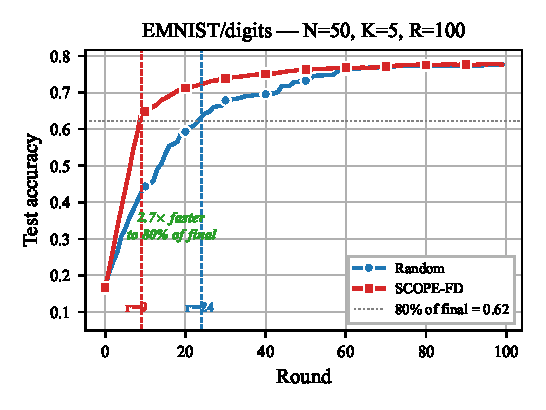
\includegraphics[width=\columnwidth]{figures/scope_paper/fig15_emnist_replication}
\caption{\new{Cross-dataset replication on EMNIST/digits at $N=50, K=5$ with MNIST as the public dataset. The proposed selector reaches $80\%$ of its final accuracy at round $9$ against random's round $24$.}}
\label{fig:emnist}
\end{figure}

\new{The corresponding accuracy trajectories are plotted in Fig.~\ref{fig:emnist}. \rev{The proposed selector reaches $80\%$ of its own final accuracy at round $9$ against round $24$ for uniform random, and its accuracy trajectory sits at or above random's throughout the run. The participation Gini coefficient is zero on the $100$-round horizon against $0.144$ for uniform random at the same $K/N = 10\%$ ratio. The fairness behaviour reported on Fashion-MNIST in Sections~\ref{ssec:exp-ablation} to~\ref{ssec:exp-scale} therefore also holds on a dataset whose feature statistics differ substantively. This replication uses a single seed and the values are reported on that basis.}}

\rev{Two further datasets were run under the full multi-seed protocol. On MNIST as the private set the ordering matches Fashion-MNIST closely: the debt-only variant reaches $90.88 \pm 0.42$, uniform random $90.58 \pm 0.43$ and the complete score $90.50 \pm 0.56$, all three inside one standard deviation of one another, while DivFL reaches $88.48 \pm 0.43$ and SubTrunc $87.91 \pm 0.50$. The participation Gini coefficient is again $1.33\%$ against $12.16\%$ for uniform random and above $36\%$ for the two submodular methods.

To test a domain outside images the selector was also run on the Free Spoken Digit Dataset, a ten-class spoken-digit corpus represented as log-spectrograms and paired with the \texttt{AudioCNN} model. The proposed selector reaches $44.08 \pm 2.58$, the debt-only variant $43.40 \pm 1.46$, uniform random $43.38 \pm 1.44$, DivFL $41.12 \pm 2.23$ and SubTrunc $40.28 \pm 1.98$, with the participation Gini coefficient at $1.33\%$. The absolute accuracy is far below the image results because the corpus provides roughly ninety training samples per client, so the ordering of the selectors rather than the absolute level is the informative quantity here. That ordering reproduces the image result, including the finding that the complete score and the debt-only variant are statistically tied.}

\rev{\subsection{Invariance of the Fairness Guarantee}
\label{ssec:exp-invariance}

Taken together the experiments above support a stronger statement than that the proposed selector is fair. Across the $278$ completed runs the participation Gini coefficient of the proposed selector is exactly $1.33\%$ in $176$ of them, spanning twelve of the sixteen experiment families. That single value is returned under every level of data heterogeneity from $\alpha = 0.01$ to $\alpha = 5.0$ and under an independent and identically distributed partition, at every downlink SNR from $-30$ to $-10$~dB, under Laplace noise on the label histogram at every $\varepsilon$ tested and under the server-side surrogate, at both staleness windows, under every public-set identity, size and label-noise level examined, on Fashion-MNIST, MNIST and the audio corpus alike, and in all thirty cells of the coefficient grid.

The four families in which the value does move are exactly those that change the participation arithmetic itself. Varying $K$ changes the cycle length, varying $N$ and $K$ together changes the residual predicted by (\ref{eq:gini_bound}), and dropout changes which clients actually participated. Everything else leaves the coefficient untouched.

This is the behaviour Proposition~1 predicts rather than a coincidence. The participation-debt term is computed from participation counts alone, so the bound in (\ref{eq:gini_bound}) depends only on $N$, $K$ and $R$. Any perturbation that leaves those three fixed cannot move the guarantee, whatever it does to the data, the channel, the public set or the privacy mechanism. The practical reading is that the fairness property can be relied upon without re-validating it for each deployment condition, which is the property a deterministic guarantee is meant to provide and which a penalty-based or stochastic fairness objective does not offer. The one condition under which it does degrade, a hard resource constraint that renders clients unselectable, is characterised in Section~\ref{ssec:exp-channel-aware}.}

% ============================================================================
% SECTION VII: CONCLUSION
% ============================================================================
\section{Conclusion and Future Work}
\label{sec:conclusion}
This paper has proposed SCOPE-FD, a deterministic, fairness-first client selector for federated distillation over massive MIMO networks under partial participation, built on top of the FedTSKD substrate of \cite{mu2024fedtskd}. SCOPE-FD acts on the over-round composition of the selected client subset through a debt-dominated three-term score with non-negative coefficients held fixed across all configurations, inheriting the $\mathcal{O}(1/t)$ convergence bound of \cite{mu2024fedtskd} unchanged and \revIVE{driving the participation Gini to zero over every $N/K$-round window whenever $K \mid N$}. \rev{Empirically, over five seeds at the headline configuration, the participation Gini coefficient falls from $12.49\%$ under uniform random selection to $1.33\%$ while final accuracy is matched at $71.21 \pm 0.99$ against $70.99 \pm 1.38$. A four-way ablation shows that the participation-debt term supplies the whole of this fairness result and that the two information terms act on the convergence path rather than on final accuracy. The fairness advantage is invariant to the Dirichlet concentration over $\alpha \in [0.05, 5.0]$, to the downlink SNR over a $20$-dB sweep, and to the client-pool size up to $N = 200$, and it persists when $K$ does not divide $N$ and when fairness is measured over windows that do not align with a participation cycle. Against four published selectors ported into the FD pipeline, the proposed selector improves on DivFL by $1.33$ and on SubTrunc by $1.81$ percentage points, and a utility-based FL selector transferred without modification reaches only $21.14 \pm 0.60$, which measures the cost of ignoring FD's aggregation rule. The accuracy advantage is concentrated in the sparse-participation regime, and at high participation ratios uniform random selection remains competitive. Beyond accuracy, the fairness guarantee proved invariant across the campaign: the participation Gini coefficient is exactly $1.33\%$ in $176$ of the $278$ runs, spanning every level of data heterogeneity, every downlink SNR, every privacy mechanism, both staleness windows, every public-set variation and all three datasets, and it moves only where the participation arithmetic itself changes. Two limits were also identified and are stated plainly. Label histogram disclosure can be removed at no measured cost through either a Laplace mechanism or a server-side surrogate. A hard energy budget, in contrast, breaks the guarantee, because filtering clients on a criterion uncorrelated with participation debt violates the assumption of Proposition~1 that every client remains selectable. Reconciling a deterministic rotation guarantee with a hard resource constraint is left open.}

\new{
%\section{Future Work}
%\label{sec:future-work}

Several extensions are left for future investigation. The first is the integration of channel-quality and energy-budget signals as additional score terms while preserving the participation-balance guarantee of Section~\ref{ssec:participation-balance}. The second is a quantitative comparison of the local-differential-privacy upload and the server-side softmax surrogate discussed in Section~\ref{ssec:penalty-term} on the FD pipeline, including a characterization of the cold-start phase under the surrogate. The third is a tighter convergence analysis that exploits the deterministic structure of the selector to refine the FedTSKD constants $\nu_n$ and $\beta_1$ in (\ref{eq:conv_bound}). The fourth is an extension beyond image classification to other softmax-output tasks such as text classification and speech recognition, where the per-class under-prediction bonus and the class-coverage penalty transfer without modification provided the server produces softmax predictions on a shared public dataset.}
\balance
% \IEEEtriggeratref{19}
\bibliographystyle{IEEEtran}
{\setlength{\itemsep}{0pt plus 0.2ex}\setlength{\parsep}{0pt}
\bibliography{references}}

\end{document}
